\documentclass[a4paper]{article}
\usepackage{amsmath}
\usepackage{graphicx}
\usepackage[colorinlistoftodos]{todonotes}
\usepackage[hidelinks]{hyperref}
\usepackage[utf8]{inputenc}
\usepackage{wasysym}
\usepackage[a4paper,top=3cm,bottom=2cm,left=3cm,right=3cm,marginparwidth=1.75cm]{geometry}
\usepackage{gensymb}
\usepackage{float}
\usepackage{mhchem}
\usepackage{pythonhighlight}
%TC:incbib
\makeatletter
\newcommand{\ssymbol}[1]{^{\@fnsymbol{#1}}}

\usepackage{verbatim}

\newcommand{\detailtexcount}[1]{%
  \immediate\write18{texcount -merge -sum -q #1.tex output.bbl > #1.wcdetail }%
  \verbatiminput{#1.wcdetail}%
}

\newcommand{\quickwordcount}[1]{%
  \immediate\write18{texcount -1 -sum -merge -q #1.tex output.bbl > #1-words.sum }%
  \input{#1-words.sum} words%
}

\newcommand{\quickcharcount}[1]{%
  \immediate\write18{texcount -1 -sum -merge -char -q #1.tex output.bbl > #1-chars.sum }%
  \input{#1-chars.sum} characters (not including spaces)%
}



\title{\huge Searching for Dark Matter in North Yorkshire: A direct light Dark
Matter search at the Boulby Underground Laboratory\\ \bigskip  \LARGE Neutron Spectroscopy using Spherical Proportional Counter
\newline 
\includegraphics[height=6cm]{bham.png}}
\usepackage{authblk}
\author[$\ssymbol{2}$]{J. Sanders}
\author[$\ssymbol{2}$]{K. Nikolopoulos}
\author[$\ssymbol{2}$]{I. Katsioulas}
\affil[$\ssymbol{2}$]{School of Physics and Astronomy, University of Birmingham,
Birmingham, B15 2TT, United Kingdom}

\begin{document}
%TC:ignore

\maketitle
\thispagestyle

\rule{411.8pt}{1pt}
\begin{abstract}
\noindent The use of Spherical Proportional Counters (SPCs) in the direct detection of Dark Matter has resulted in the requirement to remove background neutrons from the environment. The SPC has previously been validated for use in neutron spectroscopy at low pressures. This study shows the feasibility of neutron detection at pressures up to 2\,bar to reduce the impact of the wall effect on the recorded neutron energies. Using the \ce{^{14}N}(n,p)\ce{^{14}C} reaction, the detection efficiency for thermal neutrons has been calculated to be approximately $10^{-4}$ for pressures at 1, 1.5 and 2\,bar, which is an improvement from previous studies. To achieve this, data analysis was performed on the collected data to remove the majority of the noise through cuts, to leave only the neutron peak remaining. 
\newline\linebreak
\newline\textbf{Student ID:} 1777911
\newline\textbf{Key Words:} NEWS-G, Spherical Proportional Counter, WIMP, Dark Matter,Neutron Spectroscopy, Wall Effect
\newline\textbf{Word Count:} Sum count: 8601, Words in text: 7846, Words in headers: 87, Words outside text (captions, etc.): 668. Not including cover page, references and appendix.
\end{abstract}


%TC:endignore
\rule{411.8pt}{1pt}
\newpage
\setcounter{page}{1}
\tableofcontents
\newpage
\boldmath
\section{Introduction and Motivation}
During red-shift measurements of the Coma galaxy in 1933 by Fritz Zwicky, it was noted that the measured density in the region using the Doppler method was 400 times more than the density derived from the visible material \cite{andernach2017english}. Zwicky noted that this missing mass, which he termed "Dunkle Materie" (translating as Dark Matter), would have greater density than normal Matter. However due to the inaccuracy of the Hubble Constant, his calculation was incorrect by more than an order of magnitude. Despite this, his discovery formed the beginning of the study of Dark Matter \cite{richmond}. From more recent observations of the Universe, the density of Cold Dark Matter has been measured as $\Omega_ch^2 = 0.120 \pm  0.001 $, compared to the density of baryonic Matter $\Omega_bh^2 = 0.0224 \pm 0.0001 $ \cite{2020}.
\newline The density of Dark Matter has been measured to within a good uncertainty, but the nature of Dark Matter has eluded scientists for nearly 90 years. Candidates such as Weak Interacting Massive Particles (WIMPS) with  masses in the 10\,GeV - 1\,TeV mass range have been predicted through a number of models, including supersymmetry \cite{cern}. However there is evidence that the predictions of supersymmetry fails within this mass range, suggesting possibilities of lighter Dark Matter candidates \cite{Buchmueller:2012hv}.
\newline There are a number of ways to go about detecting these unknown particles: though creation at particle detectors, indirect detection and direct detection. Since 2008 the ATLAS and CMS detectors have been searching for new particles produced from proton-proton collisions by looking for missing momenta. As of yet, they have been unsuccessful in finding particles that do not fit within the standard model \cite{lopes_2020}. Indirect detection looks for an excess of standard model particles from Dark Matter annihilations and/or decays that could be found in the galaxy halo or close to black holes. These indirect searches have focused on searching within the 10\,GeV - 100\,GeV mass range, where again there is little evidence for proposed particles \cite{leane2020indirect}. Direct detection sets out to detect Dark Matter candidates from the galaxy halo using the nuclear recoil of a target nuclei. Recent developments in efficiency at low energy thresholds have allowed the search for sub 10\,GeV candidates. Most experiments using this method use noble liquids or gases but can differ in detection methods. Collaborations such as XENON use scintillation methods whereas NEWS-G uses proportional counter methods \cite{Aprile_2014,BROSSARD2019412}.
\subsection{Detector and Collaboration Background}
The Spherical Proportional Counter (SPC) was first proposed in 2008 as a multipurpose detector for the detection of alphas, neutrons and gammas \cite{Giomataris_2008}. It consisted of a prototype detector made from a copper sphere of diameter 1.2\,m with a central anode of 1.4\,cm. The reason for its development was for its ability to contain a large amount of target mass, with sub-keV energy threshold allowing for lighter and rarer particles to be detected. 
\newline Initial results came from the SEDINE detector located at the Modane Underground Laboratory in France, consisting of a 60\,cm diameter, pure copper sphere with a 6.3\,mm diameter central anode filled with a gas mixture of neon and \ce{C}\ce{H_4}\cite{Arnaud_2018}. The combination of gases was selected to fulfil the experimental criteria. A Noble gas was selected for its significant multiplication at reasonable voltages. However, due to the photons produced from the de-excitation of target atoms, the gain for pure noble gas detectors is limited. This was overcome by adding \ce{C}\ce{H_4}, allowing for gains of up to $10^6$ compared to around $10^3$ with a pure noble gas\cite{fernow_1986}. The poly-atomic gas has multiple energy levels allowing for the absorption of these photons. Figure \ref{fig:Dark} shows results from several experiments mainly centred in the energy range $3-10$\,Gev with few experiments with low mass sensitivity. The NEWS-G collaboration have set a constraint of $4.4 \times 10^{-37} cm^2$ for a WIMP mass of 0.5 $GeV$ which is shown by the solid red line. Before these results in 2018 the CRESST 2015 direct detection experiment was one of the only experiments to have a mass sensitivity of 0.5GeV \cite{Angloher_2016}.
\begin{figure}[H]
    \centering
    \includegraphics[height=8cm]{Dark.png}
    \caption{Constraints of Cross Section vs Mass for several recent experiments\cite{Arnaud_2018}.}
    \label{fig:Dark}
\end{figure}
\noindent The New Experiments With Spheres-Gas (NEWS-G) collaboration has set out to look for Dark Matter candidates in the 0.1-10\,GeV mass range.
\subsection{Project Work} \label{Project}
During direct Dark Matter detection, the background interactions within the detector volume have to be understood or completely removed. There is a large contribution from neutrons originating from two sources. One source is cosmic rays interacting with both the atmosphere and ground \cite{10.2307/984841,saxena}. Atmospheric neutrons have been measured to a reasonable degree of uncertainty \cite{flux}, which would usually dominate experiments looking for weak interacting particles. This has been negated by placing detectors such as SEDINE in underground laboratories. However placing detectors in these underground laboratories surrounds them in the second source of background neutrons, which originate from the rock produced by Uranium-Thorium traces \cite{TZIAFERI2007326}. Shielding these neutrons is difficult, so studying how neutrons interact with the detector will allow for the separation from WIMP candidates.
\begin{figure}[H]
    \centering
    \includegraphics[height=6cm]{Cross.png}
    \caption{Measured neutron cross section for the \ce{^{3}He}(n,p)\ce{^{3}H} interaction at neutron energies $10^{-4}$\,eV to 10\,MeV \cite{hnps2579}}
    \label{fig:cross1}
\end{figure}
\noindent Most commercial neutron detectors consist of a cylindrical geometry usually filled with a target mass of helium due to its large cross section, as shown in Figure \ref{fig:cross1}. However the cylindrical geometry has a large wall surface area compared to its volume, which is not optimal for spectroscopy due to the wall effect (as explained in s
Section \ref{wall}). An SPC has a much greater volume compared to its wall surface and has successfully been used for neutron spectroscopy using the \ce{^{3}He}(n,p)\ce{^{3}H} interaction \cite{hnps2579}. To reduce the wall effect, higher pressures have to be used, resulting in a greater amount of helium. However due to limited supply and high demand this would be costly, so \ce{^{14}N} is used as an alternative. Even though the cross section for neutrons with helium is higher, it is comparable with the cross section of nitrogen, as shown in Figure \ref{fig:cross}. This shortfall is improved with higher pressures, resulting in greater target nuclei in the volume for the neutrons to interact with and this has previously been carried out using the \ce{^{14}N}(n,p)\ce{^{14}C} interaction at 400\,mbar. \cite{BOUGAMONT201710}. 
\newline The aims of this project were to characterise the detector using pure nitrogen gas, and to demonstrate the feasibility of neutron spectroscopy at higher pressures.
\begin{figure}[H]
    \centering
    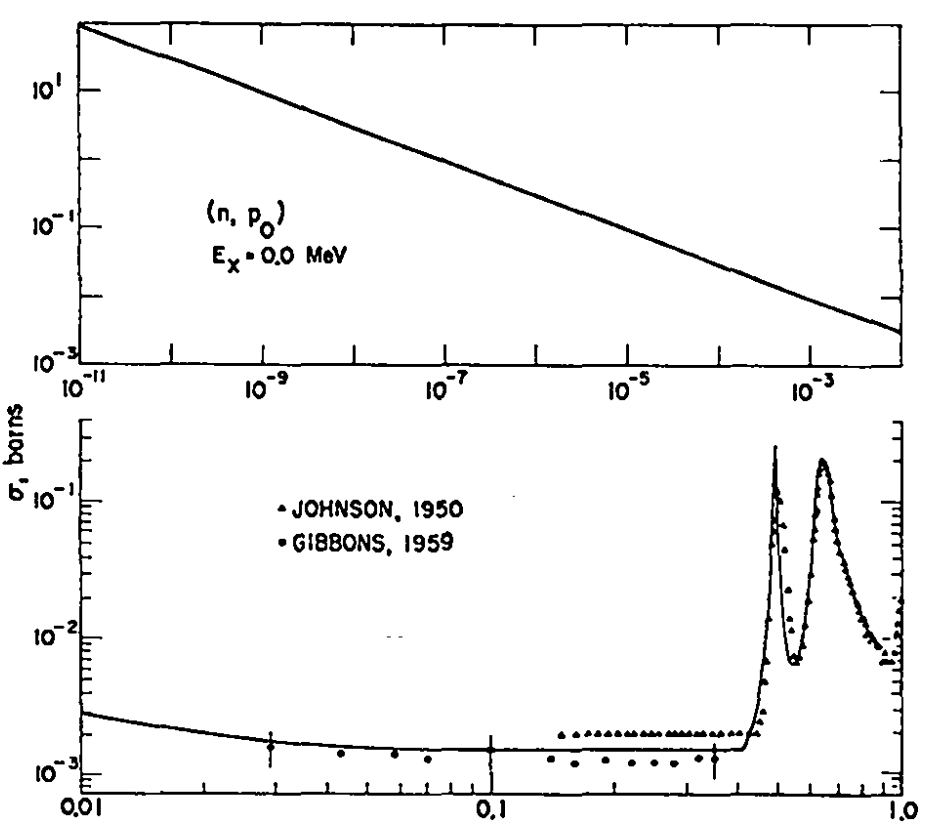
\includegraphics[height=8cm]{Crosssection.png}
    \caption{Measured neutron cross section for the \ce{^{14}N}(n,p)\ce{^{14}C} interaction at neutron energies $10^{-5}$\,eV to 1\,MeV \cite{young_foster_1972}}
    \label{fig:cross}
\end{figure}
\newpage
\section{Spherical Proportional Counter}
\subsection{Sphere}
The detector consists of a grounded 30\,cm stainless steel sphere with a central anode atop a grounded rod, as shown in Figure \ref{fig:sphere}. The gas within the volume was first evacuated using a vacuum pump, which operated overnight. The sphere was then filled with nitrogen gas to the desired pressures. 
\begin{figure}[H]
    \centering
    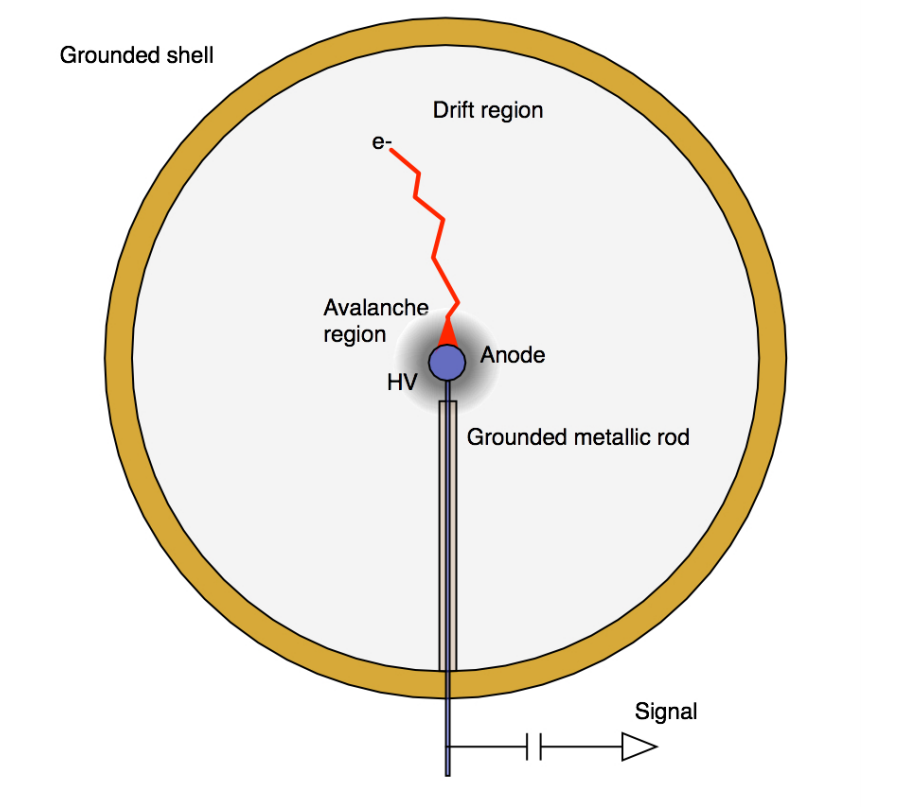
\includegraphics[height=7cm]{sphere.png}
    \caption{Diagram describing the Spherical Proportional Counter (SPC) showing the sphere wall, central anode and how an electron moves within the volume of the detector\cite{savvidis2017low}}
    \label{fig:sphere}
\end{figure}
\noindent The central anode has a bias voltage $v_0$ applied across it, which ideally produces an electric field with dependence $1/r^2$ which can be described by equation:
\begin{equation}
    E(r) = \frac{V_0}{r^2}\frac{1}{\frac{1}{r_2}-\frac{1}{r_1}}
\end{equation}
The electric field also depends upon the central anode radius $r_2$ and the radius of the sphere $r_1$. The electric field produces a drift region within the detector volume due to the voltage difference of the anode and the sphere acting as a cathode. When an incident particle interacts with the gas it ionises and produces ion pairs along a path through the volume. The ions drift towards the cathode (sphere wall) and the electrons drift towards the central anode. As the electrons drift towards the anode, their kinetic energies increase as the electric field becomes stronger, and within a few millimetres of the anode, the electric field becomes strong enough for secondary ionisations to occur. Figure \ref{fig:avala} describes how this process occurs with the electric field producing an avalanche region where multiplication can occur. It is important that avalanches are proportional to the number of electrons produced from the ionisation track in order to obtain energies describing the incident particle. This can then be characterised using the gain of the detector which has been calculated in Section \ref{gain}.
\begin{figure}[H]
    \centering
    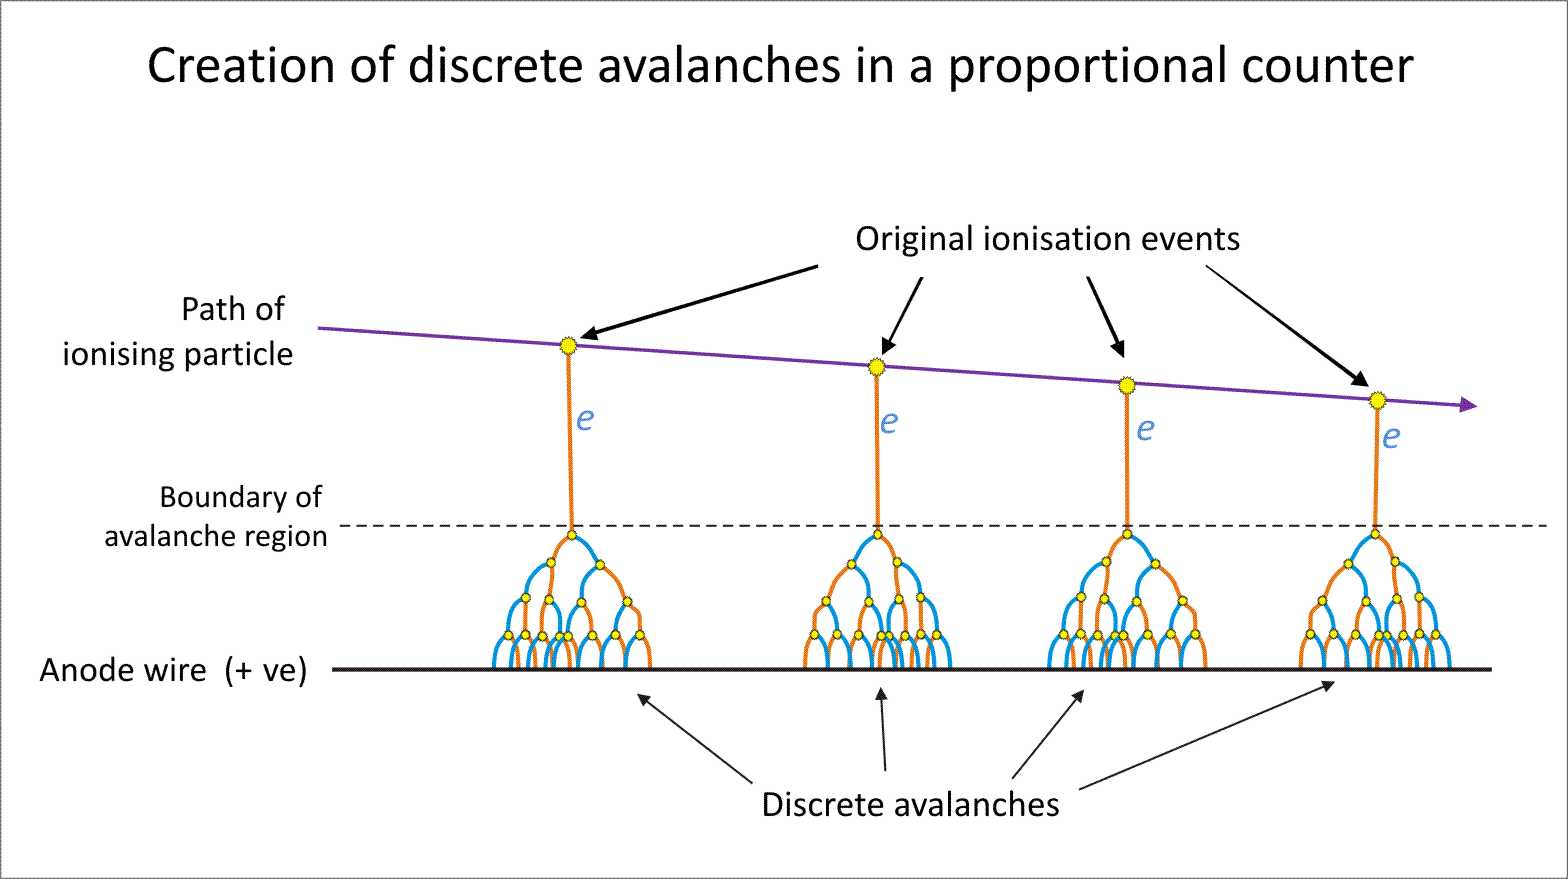
\includegraphics[height=7cm]{avalanches.jpg}
    \caption{Diagram describing how the electrons multiply within an electric field produced by an anode wire \cite{wikipedia_2021}}
    \label{fig:avala}
\end{figure}
\noindent However due to the long ionisation tracks shown in Figure \ref{fig:avala}, it is possible for the incident particle to reach the wall of the detector before dissipating all of its energy in the volume, resulting in an incomplete estimation of the particle's energy. This is known as the wall effect and has been one of the main reasons for developing a high pressure SPC neutron detector.
\subsubsection{Wall Effect} \label{wall}
The wall effect is a process where the incident particle does not dissipate all of its energy within the detector volume, would lead to an incorrect estimation of the neutron energy which is problematic for spectroscopy. In terms of neutron detection, it occurs when the proton or carbon atom reaches the wall without dissipating it's full energy in the volume. However, the proton travels much further than the carbon. If the energy is first dissipated into the wall before the neutron enters the detector volume it is hard to mitigate and would have to be understood in the final acquired data to have a complete picture of the neutrons interaction with the detector.
The interaction with the wall at end of the track can be reduced or even removed completely by increasing the number of target nuclei in the path of the incident particle, which can be achieved by increasing the pressure. For thermal neutrons, the proton's range at 500\,mbar is around 2.2\,cm \cite{katsioulas_2016}, which produced a wall effect of 2\,\%. This could be further reduced by increasing the pressure to 2\,bar, thereby increasing the number of target nuclei in the path of proton. 
\begin{figure}[H]
    \centering
    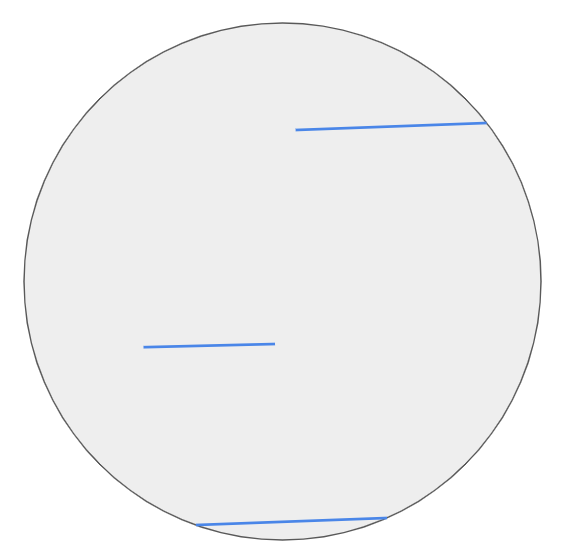
\includegraphics[height=5cm]{walll.png}
    \caption{Diagram showing examples of incident particles interacting with the detector volume and detector wall, with the blue lines describing the ionisation tracks.}
    \label{fig:wall}
\end{figure}
\noindent The percentage wall effect is low when detecting thermal neutrons but does increase significantly with higher energy neutrons producing longer ionisation tracks. 
\subsection{Achinos} \label{Ach}
Previous detectors used a single anode at the centre of the sphere shown in Figure \ref{fig:sphere}, but for large detectors or detectors operating at high pressures it was found that there was an increased probability of recombination due to the relative strength of the electric field compared to the pressure. Using the single anode, it was possible to reduce the chance of recombination by either increasing the voltage bias across the anode and/or increasing the size of the anode which in turn increased the gain. This could only be increased to a point, before the probability of electric discharge became too great and made detecting physical events difficult. 
\newline Achinos was developed by the NEWS-G collaboration to increase electric field without increasing the probability of electrical discharge. Presented in Figure \ref{fig:achinos}, it consists of 11 $\diameter$\footnote{$\diameter$-Diameter} 1\,mm anodes equidistant from the central $\diameter$36\,mm, Diamond Like carbon (DLC) coated sphere which is held in place by a grounded rod. 
\begin{figure}[H]-
    \centering
    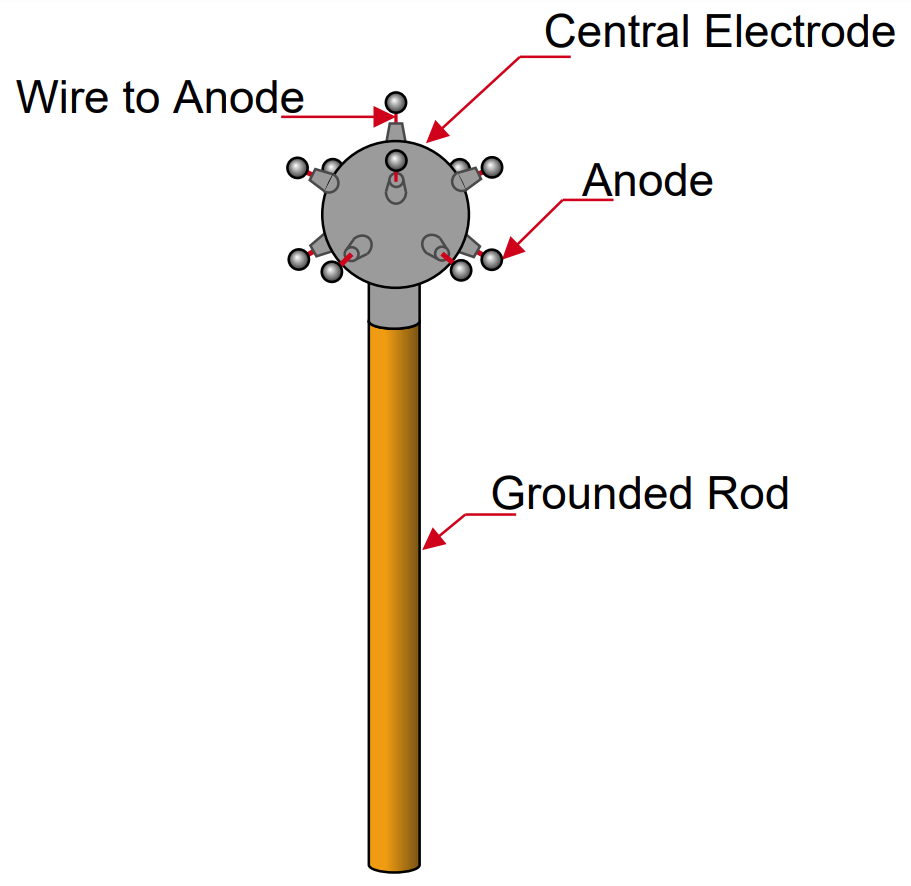
\includegraphics[height=5cm]{achinos.png}
    \caption{Diagram of Achinos sensor, comprising of 11 anodes surrounding a central sphere, atop a grounded rod \cite{Giomataris_2020}}
    \label{fig:achinos}
\end{figure}
\noindent The Achinos sensor produces eight times the electric field at large radii compared to a single $\diameter$  2\,mm anode \cite{Giganon_2017}. Currently the top six anodes are connected to a single channel named "far", in relation to the grounded rod and the bottom 5 are connected together in the channel called "near". The sensor is handmade and has imperfections in the anodes size and shape, which results in the gain across the number of anodes having variations of up 25\% \cite{Giomataris_2020}. This causes artefacts when plotting the amplitudes of pulses because of the multiple anodes on a single channel, which is described later in the results section. These artefacts will be clearer when all 11 anodes are connected on separated channels, also allowing for 3D spatial reconstruction of the ionisation track produced by the incident particle. For future experiments a 60 anode sensor is currently in development. 

\section{Detector Setup}
\subsection{Electronics}
The electronics used in the operation of the detector are shown in Figure \ref{fig:elec}.
\begin{figure}[H]-
    \centering
    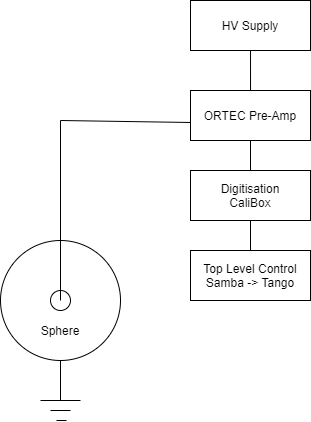
\includegraphics[height=4cm]{elec.png}
    \caption{Diagram describing the electronics used during the experiment.}
    \label{fig:elec}
\end{figure}
\subsubsection{HV supply and Pre-amp}
The high voltage supply is controlled using a computer program that allows for the fine control of voltage. It is important that when increasing the voltage, it increases at a steady rate to reduce the chance of electrical discharge, achieved by taking breaks at 100-200V intervals for the voltage to stabilise. This can be controlled remotely using team-viewer and allows for four channels of high voltage, of which two were used in this experiment.
\begin{figure}[H]-
    \centering
    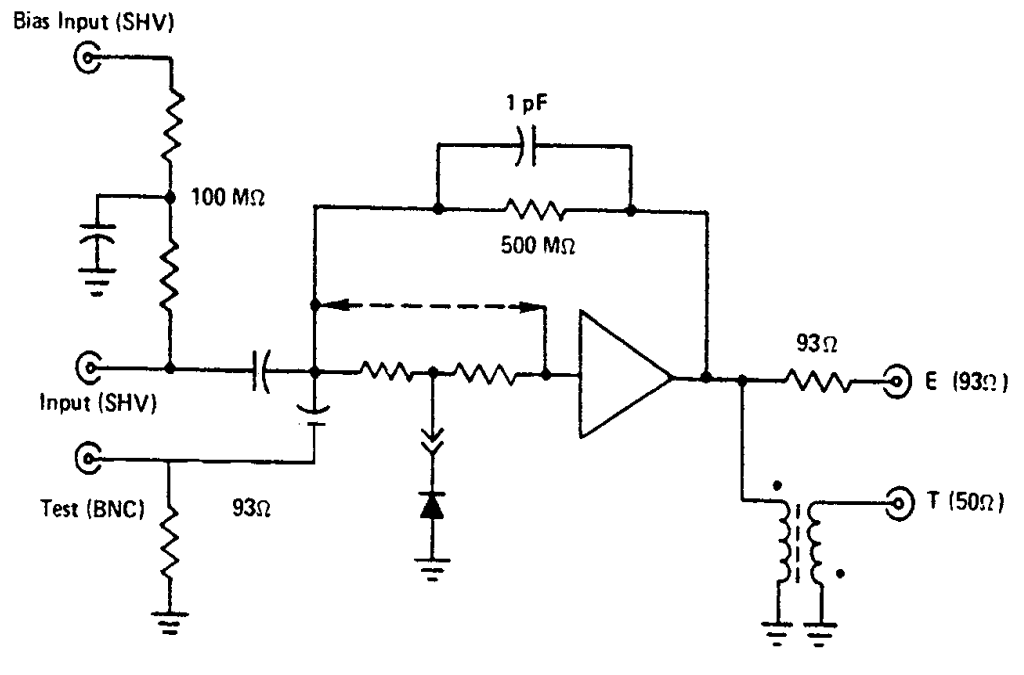
\includegraphics[height=5cm]{amp.png}
    \caption{Block Diagram of electronics used in ORTEC 142AH pre-amplifier \cite{ortec}}
    \label{fig:amp}
\end{figure}
\noindent To allow for a single cable to be used for detection and voltage bias, the pre-amplifier uses AC coupling. This is shown in Figure \ref{fig:amp} where the voltage bias is coupled to the amplifier using the front capacitor and then the input is connected to multiple anodes. It is important that the smallest length cable is used to reduce the capacitance, reducing the amount of noise produced from the pre-amplifier. The pre-amplifier is charge sensitive from the capacitor connected across the amplifier which produces the front part of the pulse in Figure \ref{fig:amplifier}. The resistor across the capacitor produces the exponential fall of around $500\,\mu s$ \cite{ortec_web} shown in Figure \ref{fig:amplifier}. 
\begin{figure}[H]-
    \centering
    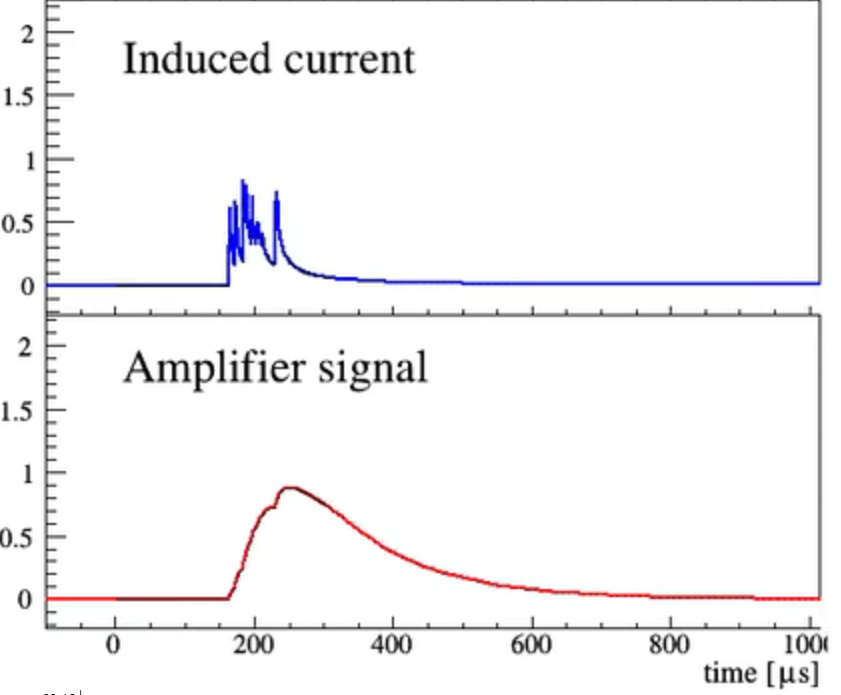
\includegraphics[height=5cm]{amplifier.png}
    \caption{Simulation of induced current on detector and output from the pre-amplifier \cite{news_2020}}
    \label{fig:amplifier}
\end{figure}
\subsubsection{Digitisation and Top level control}
The Cali box carried out the conversion from analogue to digital and is connected to a Mac computer for control and acquisition using Samba which allows for live monitoring and triggering to reduce the noise and data file sizes. Pulse shape analysis was carried out using the offline software Tango, outputting ntuple\footnote{ntuple-Tabular file format} files for later analysis using Python.
\subsection{Pulse Shape Analysis} \label{pulse}
Several characteristics can be determined from the pulses shown in Figure \ref{fig:peak}:
\begin{itemize}
    \item {\textbf{Amplitude} - Height of the pulse}
    \item {\textbf{Rise time} - Time taken for the pulse to rise from 10\% to 90\%}
    \item {\textbf{Fall} - Exponential fit of the falling edge of the pulse}
    \item {\textbf{Width} - FWHM of the pulse}
    \item {\textbf{Ratio} - $\frac{\textbf{Width}}{\textbf{Amplitude}}$} normalised.
\end{itemize}
\noindent The amplitude and rise time are affected by the incident particle and its energy deposited in the detector volume, where as the fall is mostly affected by the electronics. Using this information, electronic noise and unwanted events in the detector can be removed. The width and ratio quantifies the relationship between the height of the pulse and the fall.
\newline Using 2D histograms, regions could be identified and isolated using cuts to remove unwanted pulses without carrying out amplitude cuts. 
\begin{figure}[H]-
    \centering
    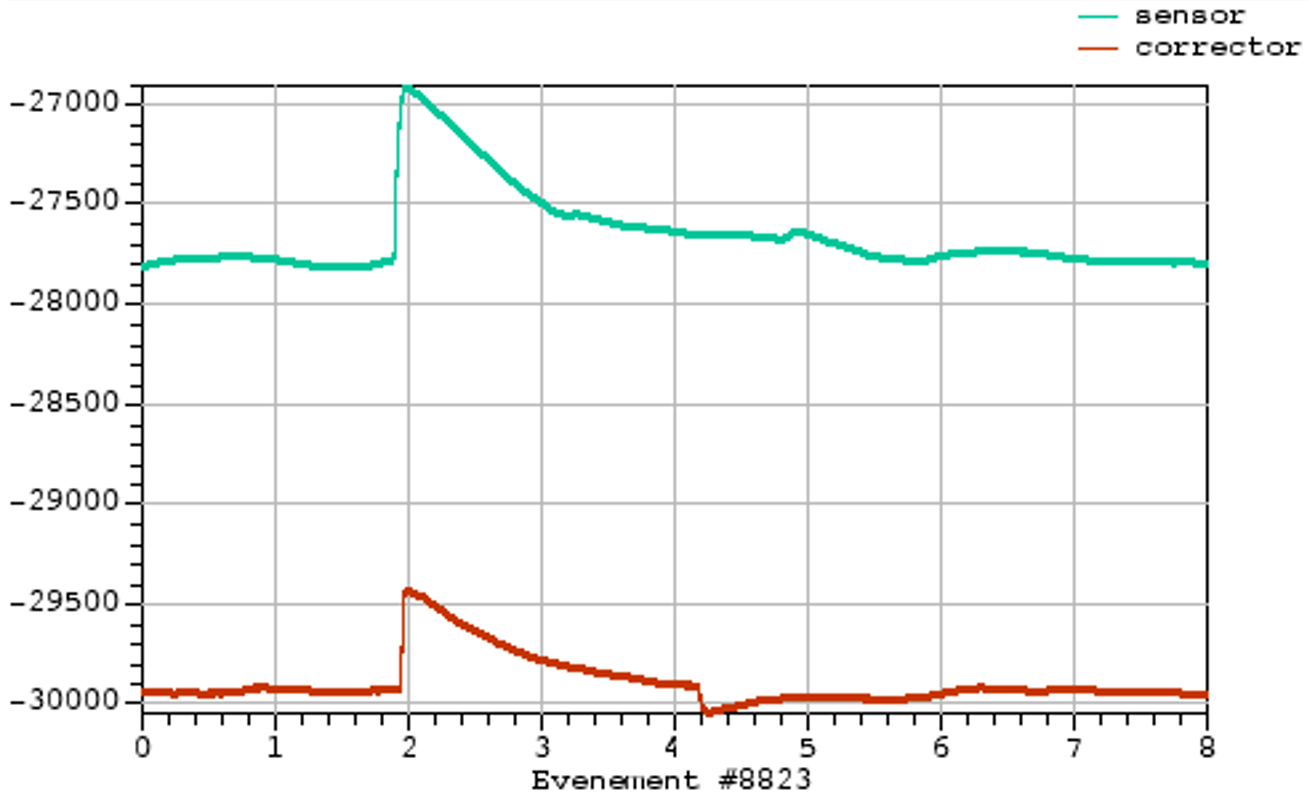
\includegraphics[height=5cm]{peak.png}
    \caption{Screen shot of two pulses triggering from the detector}
    \label{fig:peak}
\end{figure}
\subsection{Gas setup} \label{Gass}
The sphere would be first evacuated using the vacuum pump to a desired pressure of $10^{-5}$\,mbar, removing any contaminants from previous runs. It was then pumped to the specific pressure of nitrogen. The nitrogen gas was supplied by BOC and had known oxygen contaminants. As such if allowed to enter the detector with the nitrogen, it would absorb primary and secondary electrons and hence reduce the efficiency of the detector. Constant purification was carried out by the Getter filter which had radon contaminants. This however was beneficial as the radon decays over time into elements that do not affect the operation of the detector. In the short time that the radon is present in the detector it is useful as a calibration point but is still unwanted when looking for background neutrons. The time taken for the radon to decay has been studied in Section \ref{radon}.
\newline There is no need for a quencher gas, as there is no need to carry out neutron spectroscopy at very large gains, due to the higher cross section.
\begin{figure}[H]-
    \centering
    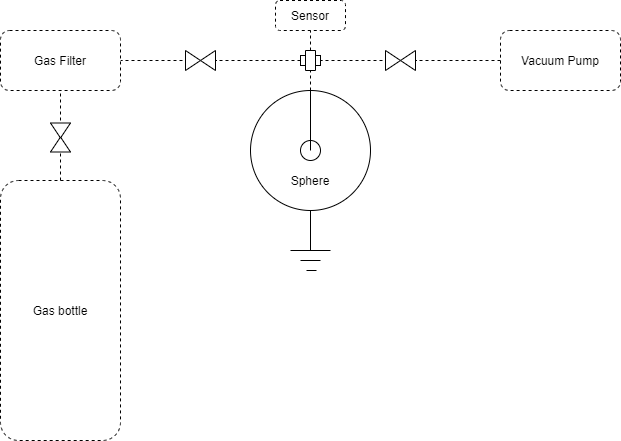
\includegraphics[height=5cm]{gas.png}
    \caption{Diagram of the gas setup used in the experiment. It comprised of a gas bottle, gas filter, pressure sensor and vacuum pump, which was controlled by a number of valves.}
    \label{fig:gas}
\end{figure}
\section{Preliminary studies}
There were several preliminary studies carried out to characterise the detector and the electronics used.
\subsection{Gain study} \label{gain}
It is important to characterise the gain of the detector to understand how the incident particle interacts within the volume of the detector and how the charges fall onto the anode. The plot in Figure \ref{fig:gain} shows the multiple regions that the detector can operate in. The first region consists of the recombination region where the electric field is not strong enough to completely separate the ions and electrons before recombining which would produce a gain of less than 1. The ionisation region is where the ions and electrons separate and are allowed to fall on to the electrodes without any multiplication, which would produce a gain of 1. The next region is where most of the experiments are carried out as it allows the original electrons to gain enough kinetic energy to cause secondary ionisations, allowing for an increased signal which is still proportional to the charge of the incident particle, producing a gain of around $1-10^5$. Beyond this region the detector operated in a limited proportional region and Geiger-Muller mode where the signals were very large but independent of the charge originally deposited in the detector volume. At these higher gains the probability of electrical discharge is high and can damage the electronics and the detector.
\begin{figure}[H]-
    \centering
    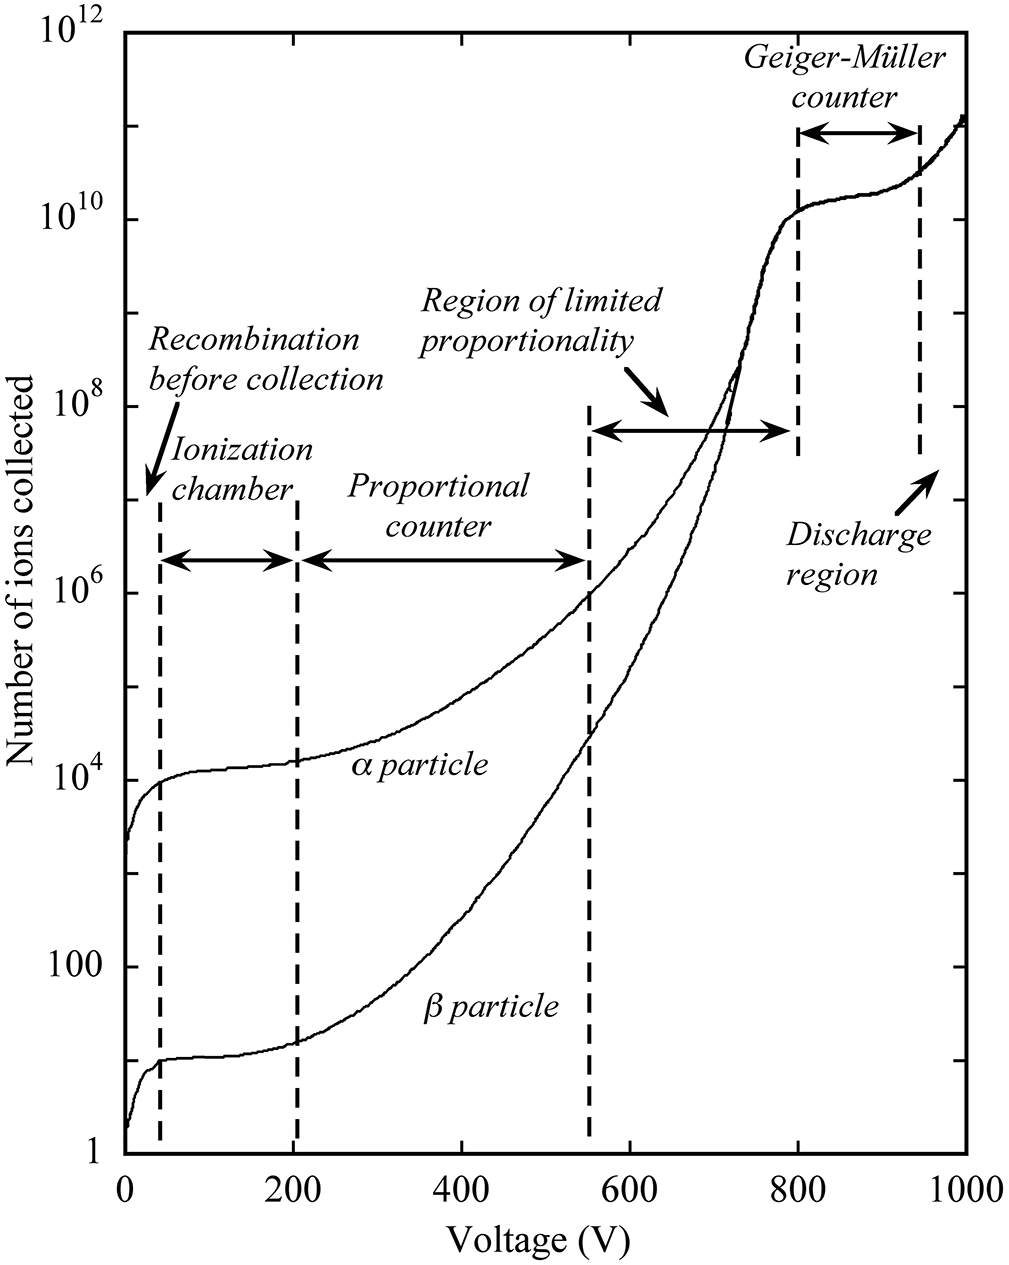
\includegraphics[height=10cm]{gain.png}
    \caption{Plot showing the number of ions collected against voltage across the anode. This describes the multiple regions that a spherical proportional counter can operate in \cite{sauli_2014}.}
    \label{fig:gain}
\end{figure}
\noindent The above Figure shows the gain increasing as the voltage bias increases across the anode, however as previously stated, the gain of the detector can be affected by a number of factors:
\begin{itemize}
    \item {Size of central anode}
    \item {Voltage bias across the anode}
    \item {Pressure of the gas in the detector volume}
\end{itemize}
\subsubsection{Method}
The gain study was carried out at, 0.5\,bar and 1\,bar with future experiments planned to be carried out at 1.5 and 2\,bar. The sphere was first opened and a sample of Americium-241 attached to a metal plate and placed at the bottom of the sphere using a magnet. The sphere was then closed and evacuated of air overnight and then pumped to the desired pressure of nitrogen. Using the known energies for the alpha decays of the sample \ref{ap:a1} the gain can be calculated using the equation \cite{Patrick}:
\begin{equation}
    G = \frac{A}{p_dp_pe\frac{E}{w}}
    \label{eq:gain}
\end{equation}
Where \textbf{A} is the amplitude of the alpha peak described by a Gaussian fit, \boldmath{$p_p$} being the voltage output per unit charge on the anode (mV/e), \boldmath{$p_d$}  the voltage to channel conversion (mV/ADU), \textbf{E} the energy of the ionising particle and \textbf{w} which is the first ionisation energy of the gas.
\newline Both {$p_p$} and \boldmath{$p_d$} are dependant on the selected pre-amplifier, which was originally a CANBERRA model but was consequently swapped to an ORTEC model.
\newline \boldmath{$p_d$} was found using the test input of the pre-amplifier shown in Figure \ref{fig:amp}. A known oscillating square wave, produced by the oscilloscope was connected to the test input and produced an amplitude peak that corresponded to the voltage which was $26.3513\,ADU/mV$. 
\newline \boldmath{$p_p$} is the conversion factor defined by the manufacturer of the pre-amplifier to be $45\,mV/MeV$ \cite{ortec}.
\subsubsection{Results-500\,mbar}
Results were first taken for 500\,mbar using the CANBERRA pre-amplifier, however as previously stated the amplifier has a small time constant which doesn't allow for the higher rise times produced from the detector before the pulse is cut off. In Figure \ref{fig:uj} the alpha peak has been separated into multiple peaks caused by the ballistic deficit, which makes the analysis difficult as it fails to follow a statistical Gaussian shape.
\begin{figure}[H]-
    \centering
    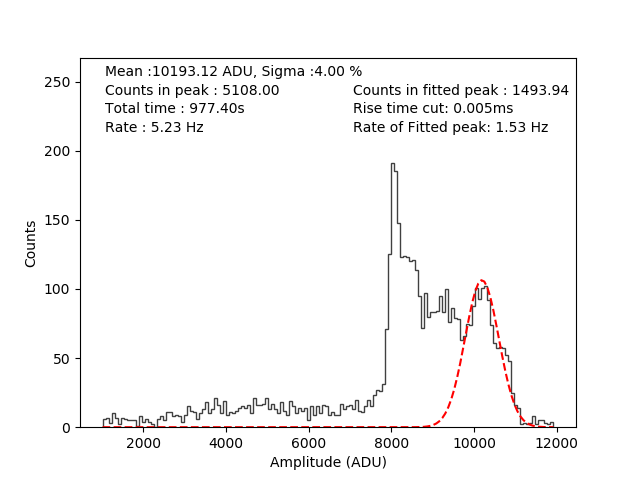
\includegraphics[height=5cm]{uj27n001_amp.png}
    \caption{Plot of Polonium 210 alpha peak, showing the ballistic deficit at 500\,mbar.}
    \label{fig:uj}
\end{figure}
\noindent For all later runs the ORTEC amplifier was used. Results were taken at 500\,mbar for several voltages between 400\,V and 2700\,V. The plot in Figure \ref{fig:uk} is an example alpha peak recorded by the analysis software which no longer has the multiple peaks shown in Figure \ref{fig:uj}. To find the amplitude of the alpha peak a Gaussian plot was taken using the equation:
\begin{equation}
    f(x) = \frac{A}{\sigma\sqrt{2\pi}}e^{-\frac{1}{2}(\frac{x-\mu}{\sigma})^2}
    \label{eq:guas}
\end{equation}
Constants \textbf{A}, \textbf{$\mu$} and \textbf{$\sigma$} were optimised using the curve fit function found in the scipy python module \cite{scipy}. The curve\_fit module produces an error for the estimated values which were used as well as experimental errors on the components of Equation \ref{eq:gain}. 
\begin{figure}[H]-
    \centering
    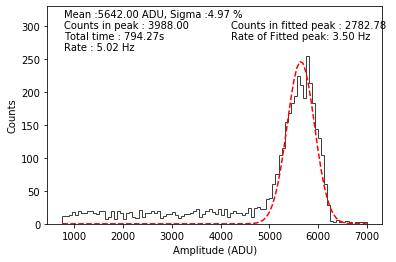
\includegraphics[height=5cm]{uk09n002_amp.png}
    \caption{Plot of Americium 241 alpha peak at 2700V for 500\,mbar.}
    \label{fig:uk}
\end{figure}
\noindent Using the means from the plotted Gaussian, the gain was calculated using equation \ref{eq:gain} and plotted against voltage in Figure \ref{fig:gain1}. In comparison with the known gain curve in Figure \ref{fig:gain}, only the proportional region and the start of the ionisation region can really been seen with the gain reaching just above 1 at 400V and increasing exponentially to around 60 at 2700V. This was the lowest voltage before the alpha peak would start to combine with the low amplitude noise peak and become unrecognisable.
\begin{figure}[H]-
    \centering
    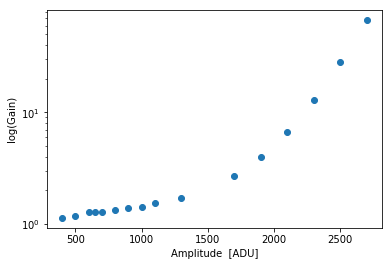
\includegraphics[height=5cm]{gain1.png}
    \caption{Plot for the gain at voltages between 2700V and 400V for 500\,mbar nitrogen}
    \label{fig:gain1}
\end{figure}
\noindent It is important to reach the ionisation region to calculate the actual \textbf{w} value for the gas rather than using a known value. As the voltage could not be lowered the only way to reach this was to increase the pressure.
\subsubsection{Results-1\,bar}
Results at 1\,bar were taken using the Polonium-210 sample located at the bottom of the sphere, decaying via alphas with energies of around 5.3\,MeV \ref{ap:a11}, producing peaks very similar to the ones in Figure \ref{fig:uk}. Figure \ref{fig:gain2} shows the gain plot at 1\,bar between 1800-3800\,V with the regions described by the three colours. At voltages between 1800-1900V the detector operates within the recombination region with a gain of less than one which is shaded in red. Voltages between 1900-2050\,V are in the ionisation region where the w value can be calculated and voltages between 2050-3800\,V are within the proportional region where the experiments for neutron spectroscopy operate.
\begin{figure}[H]-
    \centering
    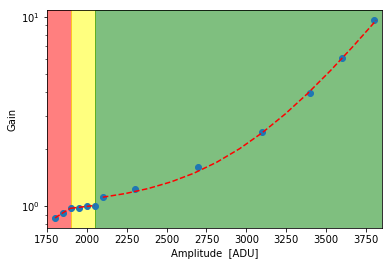
\includegraphics[height=5cm]{1bargainfit.png}
    \caption{Plot for the gain at voltages between 3800V and 1800V for 1\,bar nitrogen}
    \label{fig:gain2}
\end{figure}
\noindent The three regions can be described accurately using Equation \ref{eq:3gain} with most of the points falling on the lines. However they are not continuous around 2050V due to slight contamination of oxygen in the detector volume which lowered the gain a little between measurements.
\begin{equation}
f(x) = \begin{cases} 0.00111x-1.13539 &\mbox{for } 1800 \leq x  \leq 1900 \\
0.00022x+0.54797 & \mbox{for } 1900\leq x \leq 2050 \\
0.16317^{(x-0.99317)}+2223.74 & \mbox{for }  2100 \leq x
\end{cases}
\label{eq:3gain}
\end{equation}
 The ionisation region was selected to calculate the \textbf{w} value, as the same amount of charge is deposited on the sensor that is initially deposited in the detector volume due to other regions having an amplification factor. To calculate the \textbf{w} value for the nitrogen gas, equation \ref{eq:gain} is rearranged to form Equation \ref{eq:w},
\begin{equation}
    w = \frac{p_dp_peG}{AE}
    \label{eq:w}
\end{equation}
\noindent In Figure \ref{fig:gain2}, there are four points with a gain of 1. To find the amplitude of these points, an average was taken, $A=189.62$\,ADU, thus producing a \textbf{w} value of $36.84 \pm 0.04$\,eV, which is close to the known value for w as $36.39 \pm 0.04$ \cite{Krieger_1979}. 
\subsection{Calibration} \label{calib}
Calibration allows for the conversion of amplitude [ADU] to energy [eV], allowing for the detection of differing particles of different energies. The calibration was carried out for 1\,bar at a number of voltages. However in this report only 3800\,V will be shown and the remainder will be presented the report submitted by Sam Green \cite{green}. To calibrate the detector, multiple known energies were taken. The 5.3\,Mev alpha peak from the Americium 241 decay used in the gain study was used, as was the 625\,keV thermal neutron peak from the neutron study. If the calibration was immediately carried out after the pumping of the gas then the 5.5\,Mev radon alpha peak could be used. 
\subsubsection{Results}
The detector has two channels that can be recorded, near and far. However when using an alpha source placed at the bottom of the sphere only the far channel will produce an alpha peak due to the minimal penetration of an alpha particle. This results in only the far channel being calibrated, though in future, the source could be moved using the magnet to calibrate the other channel. 
\begin{figure}[H]-
    \centering
    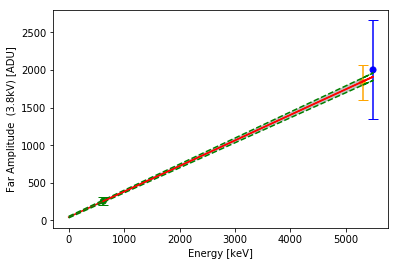
\includegraphics[height=5cm]{3800_2N.png}
    \caption{Calibration plot for 1\,bar at 3800V}
    \label{fig:cali}
\end{figure}
\noindent In Figure \ref{fig:cali}, the green point represents the 625\,keV neutron, the orange point the 5.3\,Mev Polonium peak and the blue the 5.5\,Mev radon peak. The red line follows the equation:
\begin{equation}
    y = 0.34018x + 42.9610
\end{equation}
The two dotted green lines plot the upper and lower bounds of the error produced by the curve\_fit function, used to estimate the coefficients of the $y=mx+c$ straight line. The error on the radon peak is significant due to the low count rate of the alpha peak, which could be negated in future by increasing the time of measurement. These points produced an equation to convert the amplitude to energy at 3800V on the far channel:
\begin{equation}
    E = \frac{A-42.9610}{0.34018}
\end{equation}
With the error on the energy calculated using,
\begin{equation} \label{eq:error}
    \left(\frac{\delta E}{E}\right)^2 = \left(\frac{\sqrt{(\delta A)^2 + (\delta c)^2}}{A-c}\right)^2+\left(\frac{\delta m}{m}\right)^2
\end{equation}
This is a very preliminary result and in Figure \ref{fig:cali} there is a large range of energies that have no points, meaning that the calibration is only relevant for energies close to the neutron or alpha peaks. To improve this in the future energies would have to be selected to fill this gap.
\subsection{Radon Measurements} \label{radon}
As stated in Sections \ref{Gass} and \ref{calib}, there is a presence of radon within the detector volume that was used as a third point for calibration. However, for low count rate spectroscopy this is unwanted and needs to be removed, especially for fast neutron detection which has around the same energy as the radon alpha peak.
\newline radon has a short half-life of 3.8215 days resulting in the radon peak being undetectable after a number of weeks. However this had to be checked \cite{osti_1348827}. The radon decays to Lead-210 which has a long half-life of 21 years \ref{ap:a2}. This will not interfere with the neutron experiments but would have to be investigated for use in Dark Matter detection. 
\subsubsection{Method}
As the radon has a known half-life, the count-rate will decrease to a known amount after a period of time, so two separate measurements were taken with a measured time difference. The first measurement was taken 195 minutes after gas filling and lasted for 287 mins for a total 482 mins after filling. The second measurement was taken 1862 mins after gas filling and lasted 490 mins for a total time of 2352 minutes after gas filling.
\newline A simple calculation can predict the count rate at each point in time. Take the count rate of 100 at the time of pumping of the gas, using equation \ref{eq:half}.
\begin{equation}
    N = N_0e^{(-0.693\frac{t}{t_{1/2}})}
    \label{eq:half}
\end{equation}
\noindent After 482 mins the count would reduce to 94.11 and then to 74.39 after 2352 mins which can be compared to experimental results to ensure that it was radon contributing to the count rate.
\subsubsection{Results}
The two measurements were taken at 3600V at a pressure of 1\,bar and produced the two histograms in Figure \ref{fig:radon}. The red histogram is that of the first run producing the higher rate compared to the second run, which is shown in blue. 
\begin{figure}[H]-
    \centering
    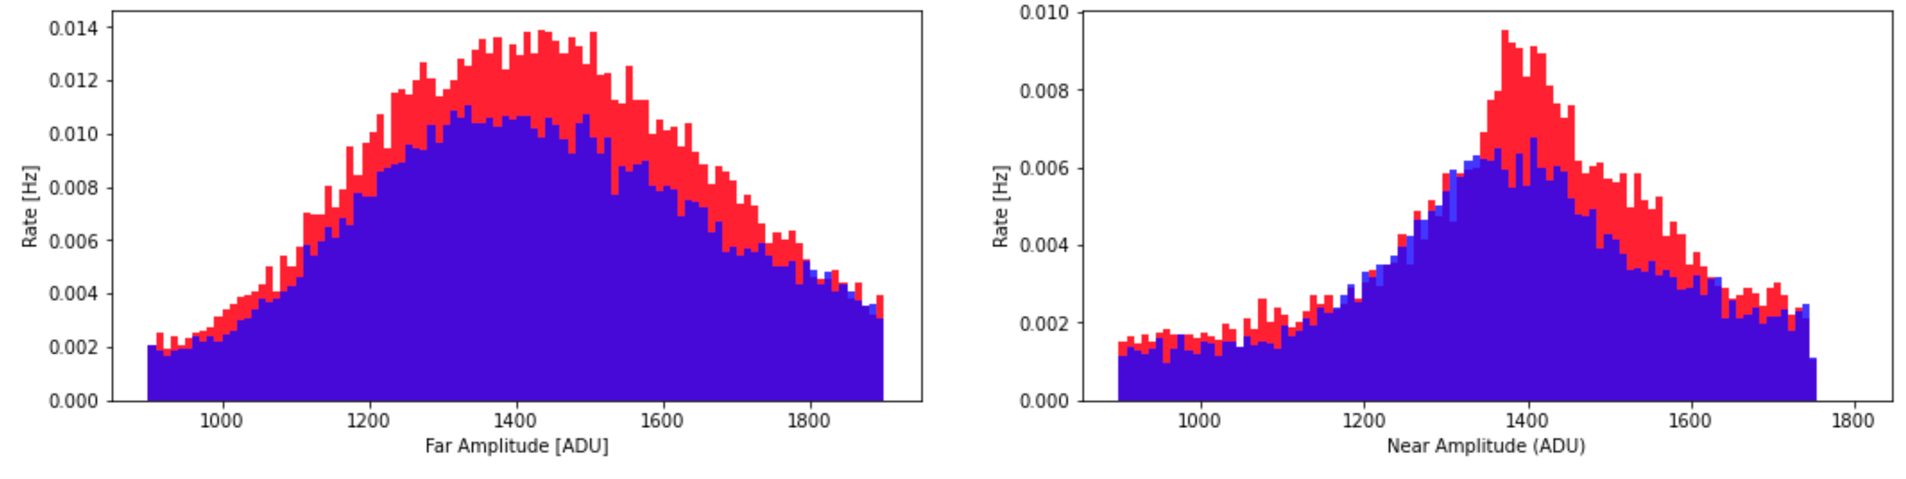
\includegraphics[height=3.5cm]{radon.png}
    \caption{Radon peaks for 1\,bar at 3600V for both the near and far channel. The Red histogram is the first run and the blue is the second run.}
    \label{fig:radon}
\end{figure}
\noindent The rate of the peak was taken by calculating the number of events within the bounds of the histogram divided by the time of acquisition. Table \ref{tb:radon} contains the final results from the two runs for both the far and near channel, as well as the predicted second run rate using the calculation set out in the method. The second run for the far channel was close to the expected rate, only deviating by 0.45\% from the expected result, but was further from the expected rate in the near channel. This suggests that the radon decay is the main contributor of this peak and would take several days for enough radon to decay to a Lead 210 for the peak to be negligible compared to the background events seen before the radon peak at around 1000\,ADU.
\begin{table}[H]-
\centering
\caption{Results validating the radon decay in the detector volume}
\begin{tabular}{|l|l|l|l|l|} 
\hline
Channel~ & \begin{tabular}[c]{@{}l@{}}First Run\\(Hz)\end{tabular} & \begin{tabular}[c]{@{}l@{}}Second Run\\(Hz)\end{tabular} & \begin{tabular}[c]{@{}l@{}}Expected Second Run\\(Hz)\end{tabular} & \begin{tabular}[c]{@{}l@{}}Variation\\(\%)\end{tabular}  \\ 
\hline
Far      & 0.834                                                   & 0.668                                                    & 0.665                                                             & 0.45                                                     \\
Near     & 0.376                                                   & 0.306                                                    & 0.297                                                             & 3.03                                                     \\
\hline
\end{tabular}
\label{tb:radon}
\end{table}
\section{Neutron Measurements}
Neutrons interact with nitrogen through two interactions, depending on its energy. For thermal and fast neutrons up to 1.7\,MeV, the interaction occurs through \ce{^{14}N}(n,p)\ce{^{14}C}:
\begin{equation}
    \ce{^{14}N} + n \rightarrow \ce{^{14}C} + p + 625.87keV
    \label{eq:neu}
\end{equation}
The proton and carbon are the particles that produce the ionisation tracts with the energy produced from the neutron interaction shared between the carbon and proton. For energies greater than 1.7\,Mev and up to 20\,MeV, the interaction \ce{^{14}N}(n,$\alpha$)\ce{^{11}B} dominates: 
\begin{equation}
    \ce{^{14}N} + n \rightarrow \ce{^{11}B} + \alpha - 158keV
\end{equation}
\subsection{Neutron Source}
The neutron source used is americium241-beryllium9 (Am-Be). Chosen for the Am alpha decay and the Be low Z, which interacts with the alpha producing a neutron \cite{nrc},
\begin{equation}
    \ce{^{9}B} + \alpha \rightarrow \ce{^{12}C} + n + 4.44MeV \gamma
\end{equation}
Which has the characteristics,
\begin{itemize}
    \item[] {Half-life: $432.2\,y$}
    \item[] {Source activity: $1\,Curie = 3.7 \times 10^{10}\,Bq$}
    \item[] {Average neutron energy: $4.2\,MeV$}
\end{itemize}
The material is held within a X3 stainless steel capsule shown in Figure \ref{fig:ambe}, with dimensions $d = 22.4\,mm$ and $h = 31\,mm$. The case decreases the neutron output for the source to $2.6 \times 10^{6}\,Bq$ but keeps the source contained. Due to the high average neutron energy it is important that the source be kept in a radiation box when not being used due to the high average energy of the neutron.
\begin{figure}[H]-
    \centering
    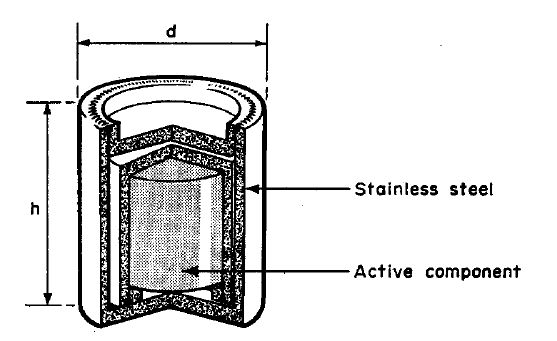
\includegraphics[height=5cm]{ambe.png}
    \caption{Diagram of Am-Be source contained within a stainless steel capsule \cite{LORCH1973585}}
    \label{fig:ambe}
\end{figure}
\subsection{Graphite Stack}
For operations in the laboratory at the University of Birmingham it is dangerous to have a neutron source with energies in the MeV range. To slow the neutrons to thermal energies, the source was placed in the centre of the graphite stack shown in Figure \ref{fig:stack}, with the graphite acting as a moderator. The graphite was selected as a moderator due to its low neutron absorption of 0.0035\,barns and its large neutron scattering cross section of 5.56\,barns \cite{taylor_francis_1992}. It is also selected for its good thermal stability, reasonable cost and the fact that it is self contained, compared to other moderators such as deuterium \cite{osti_4844185}.
\begin{figure}[H]-
    \centering
    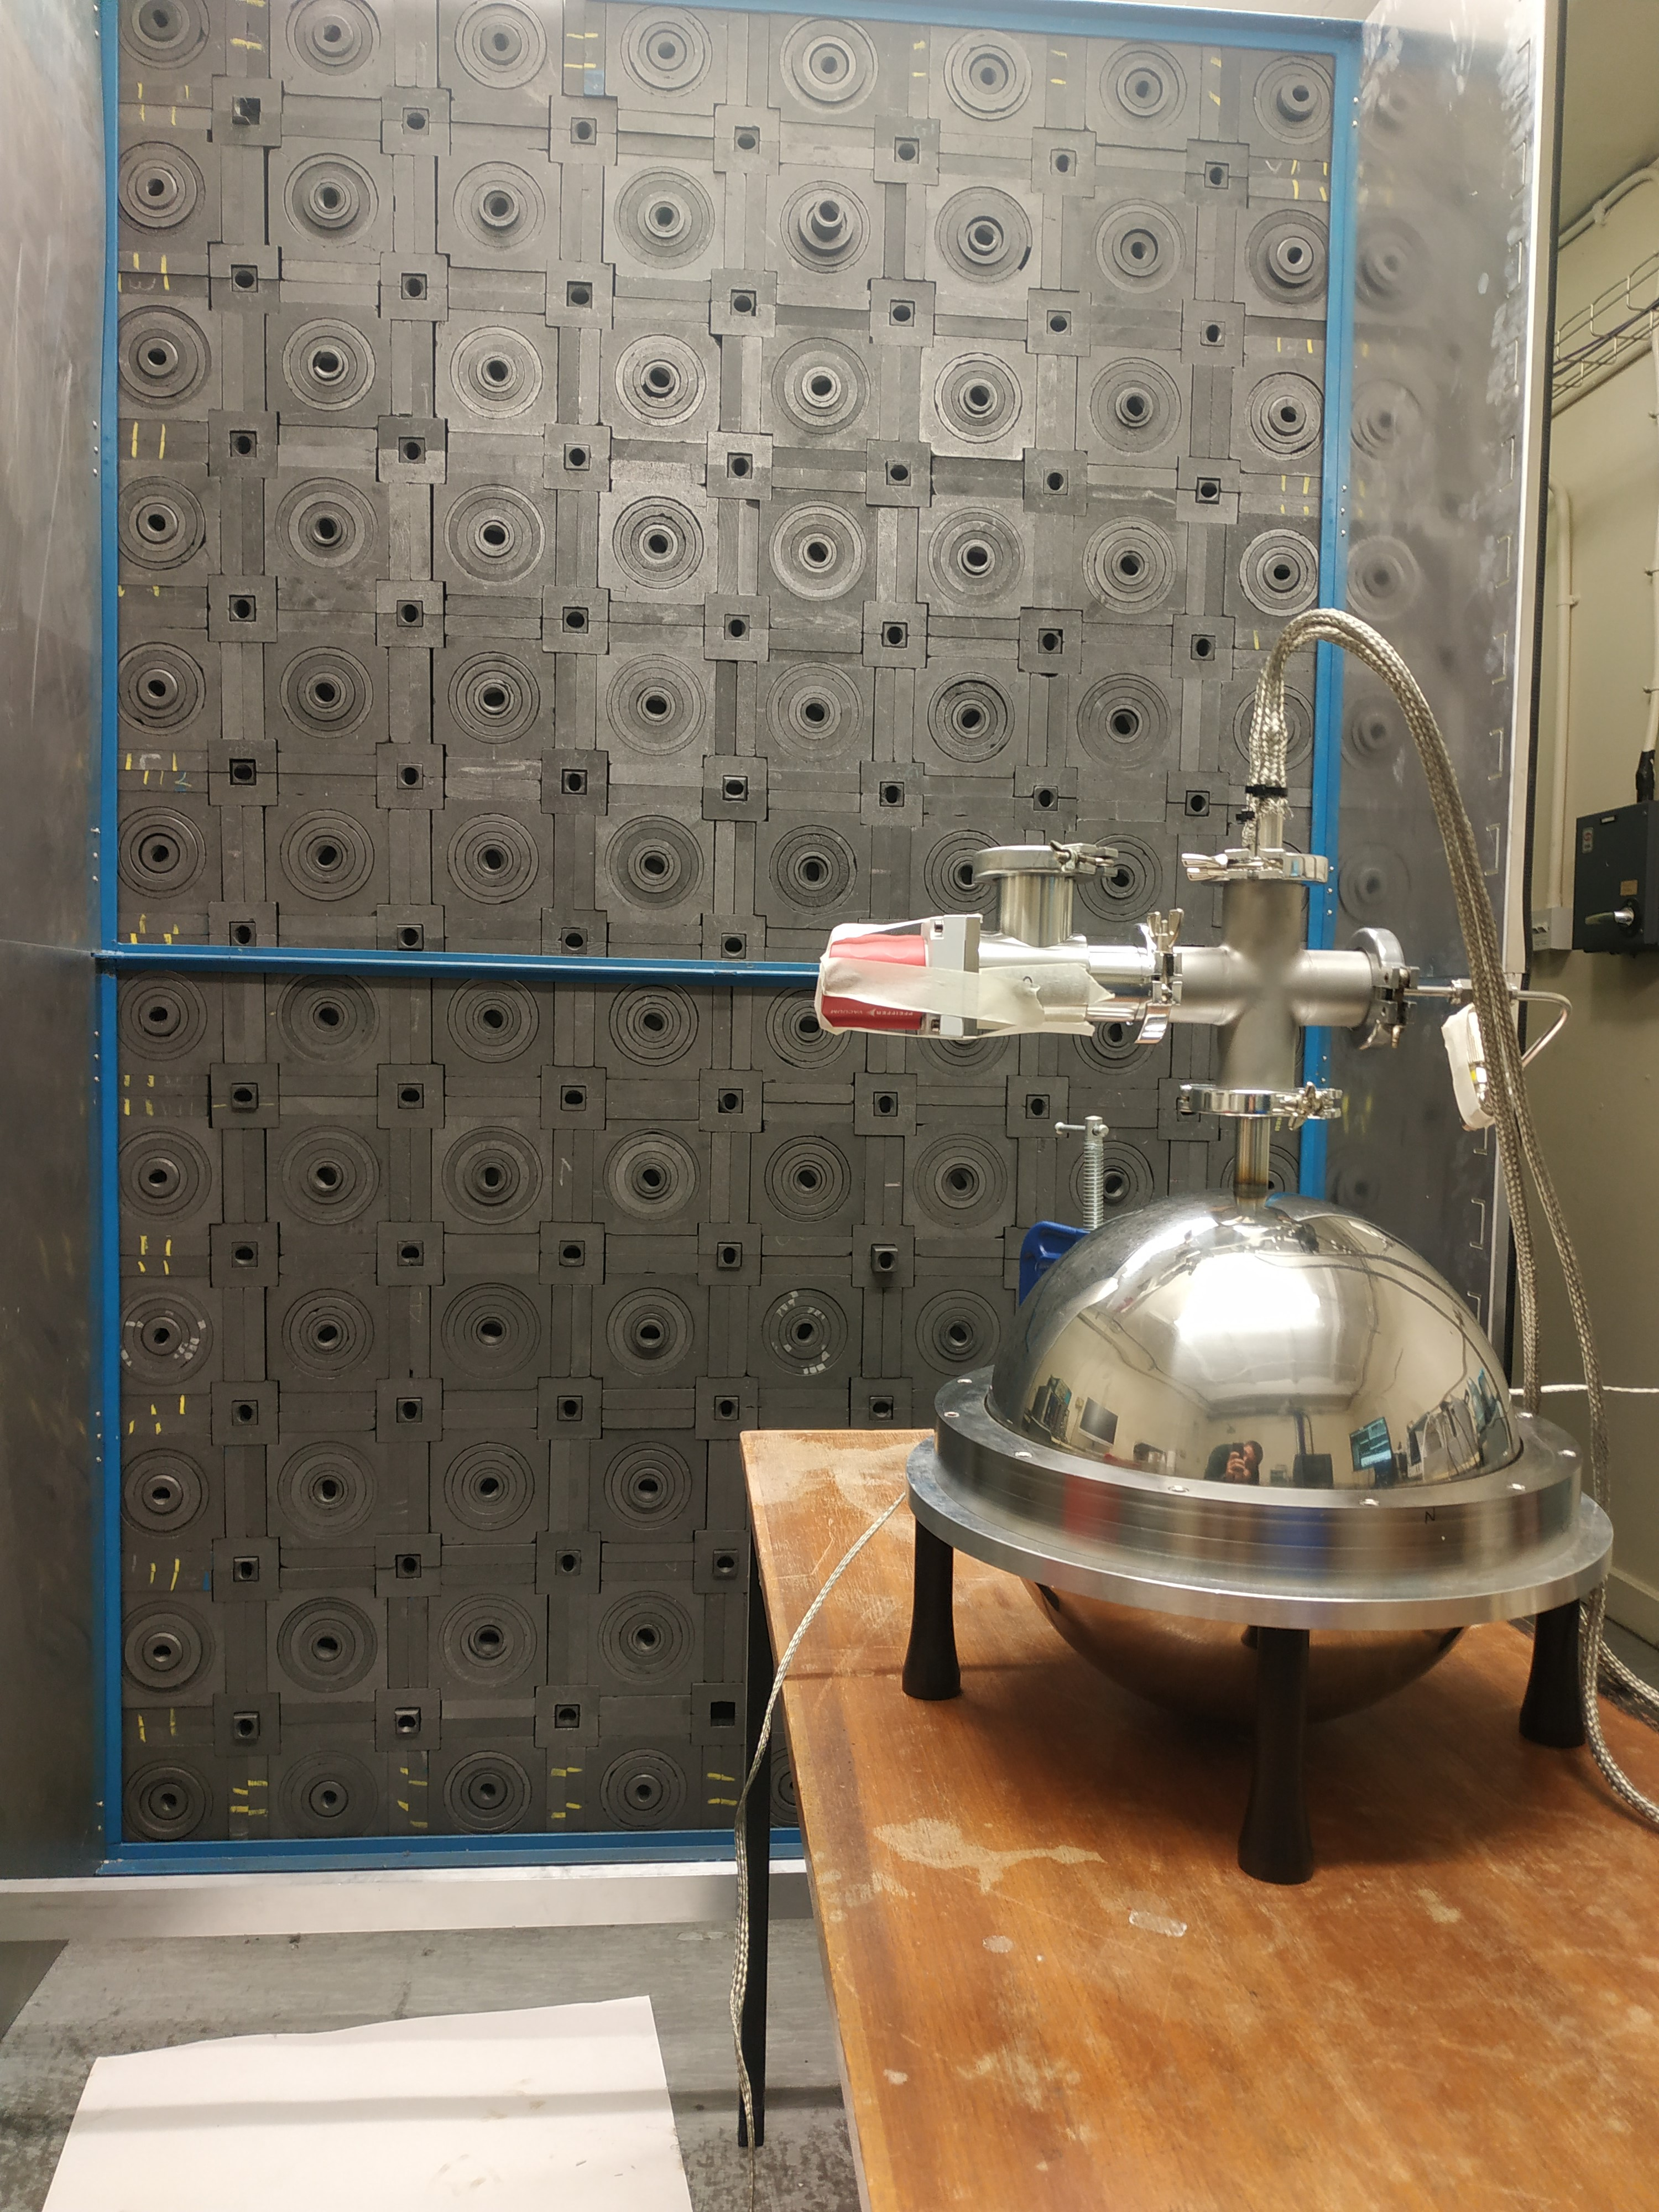
\includegraphics[height=8cm]{stack.jpg}
    \caption{Photo of graphite stack and SPC at The University of Birmingham \cite{ion}}
    \label{fig:stack}
\end{figure}
\noindent The source was placed in the centre of the graphite stack, level with the detector which was  important to know when calculating the number of neutrons passing through the detector volume.
\subsection{Method}
Neutron measurements were taken at multiple voltages at 1\,bar, but only 3800V is shown in this study. Measurements were taken at a two voltages at 1.5\,bar and one at 2\,bar.
\newline Before each measurement at different pressures the sphere was removed from the graphite stack room and taken to the lab to be evacuated of air overnight and pumped to the desired pressure of nitrogen. The sphere was taken back to the graphite stack room, with prior checks made to ensure that moving the sphere would not affect the later measurements. Each measurement was taken over a time period to collect a large number of events, allowing good statistics to be produced for the neutron peak. 
\newline The raw data acquired from the detector during a neutron measurement is shown in Figure \ref{fig:ampb}. It produces a double peak, were the large low amplitude peak is a combination of noise that was not removed from the acquisition cut and a contribution from the incident particles interacting with the wall, resulting in lower energy being recorded. The second peak is produced by the thermal neutrons, though there remains a number of expected noise events within this peak. 
\begin{figure}[H]-
    \centering
    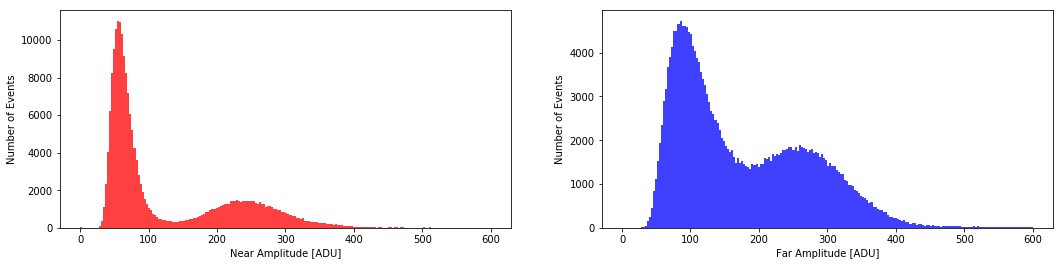
\includegraphics[height=3.7cm]{uk24n001_ampbefore.png}
    \caption{Amplitude histogram of raw data produced for 3800V at 1\,bar}
    \label{fig:ampb}
\end{figure}
\noindent To remove the noise and unwanted events, characteristics from the pulse were used as was set out in Section \ref{pulse}. Cuts were chosen by zooming into the regions of interest on the 2D histograms such as in Figure \ref{fig:1rise}. Using Python, the data outside the selected regions was cut using a 'for' loop shown in the example below.
\begin{python}
for i in range(len(amplitude_c)):
 if 0 <= len_c[i] <= 0.325 and 0.3 <= fall_c[i] <= 1.25 and 0.3 <= dur_c[i] <= 1.5 
 and 0.0075 <= rtc[i] <= 0.07 and amplitude_c[i]>=0:
\end{python}
\noindent After the cuts were made, the rate of the neutron peak was calculated and would be compared to the simulated number of neutrons that passed though the detector volume. The plot in Figure \ref{fig:prob} shows the probability of the neutrons passing through the detector volume at multiple neutron energies after passing through the graphite stack, produced using a simulation provided, of the graphite stack \cite{Ben}. Using the known activity of the source, the expected number of events passing through the detector volume can be calculated to be  $6.76 \times 10^3$\,Hz. Comparing the expected number of neutrons passing through the detector volume and the rate detected allows for a calculation of the efficiency.
\begin{figure}[H]-
    \centering
    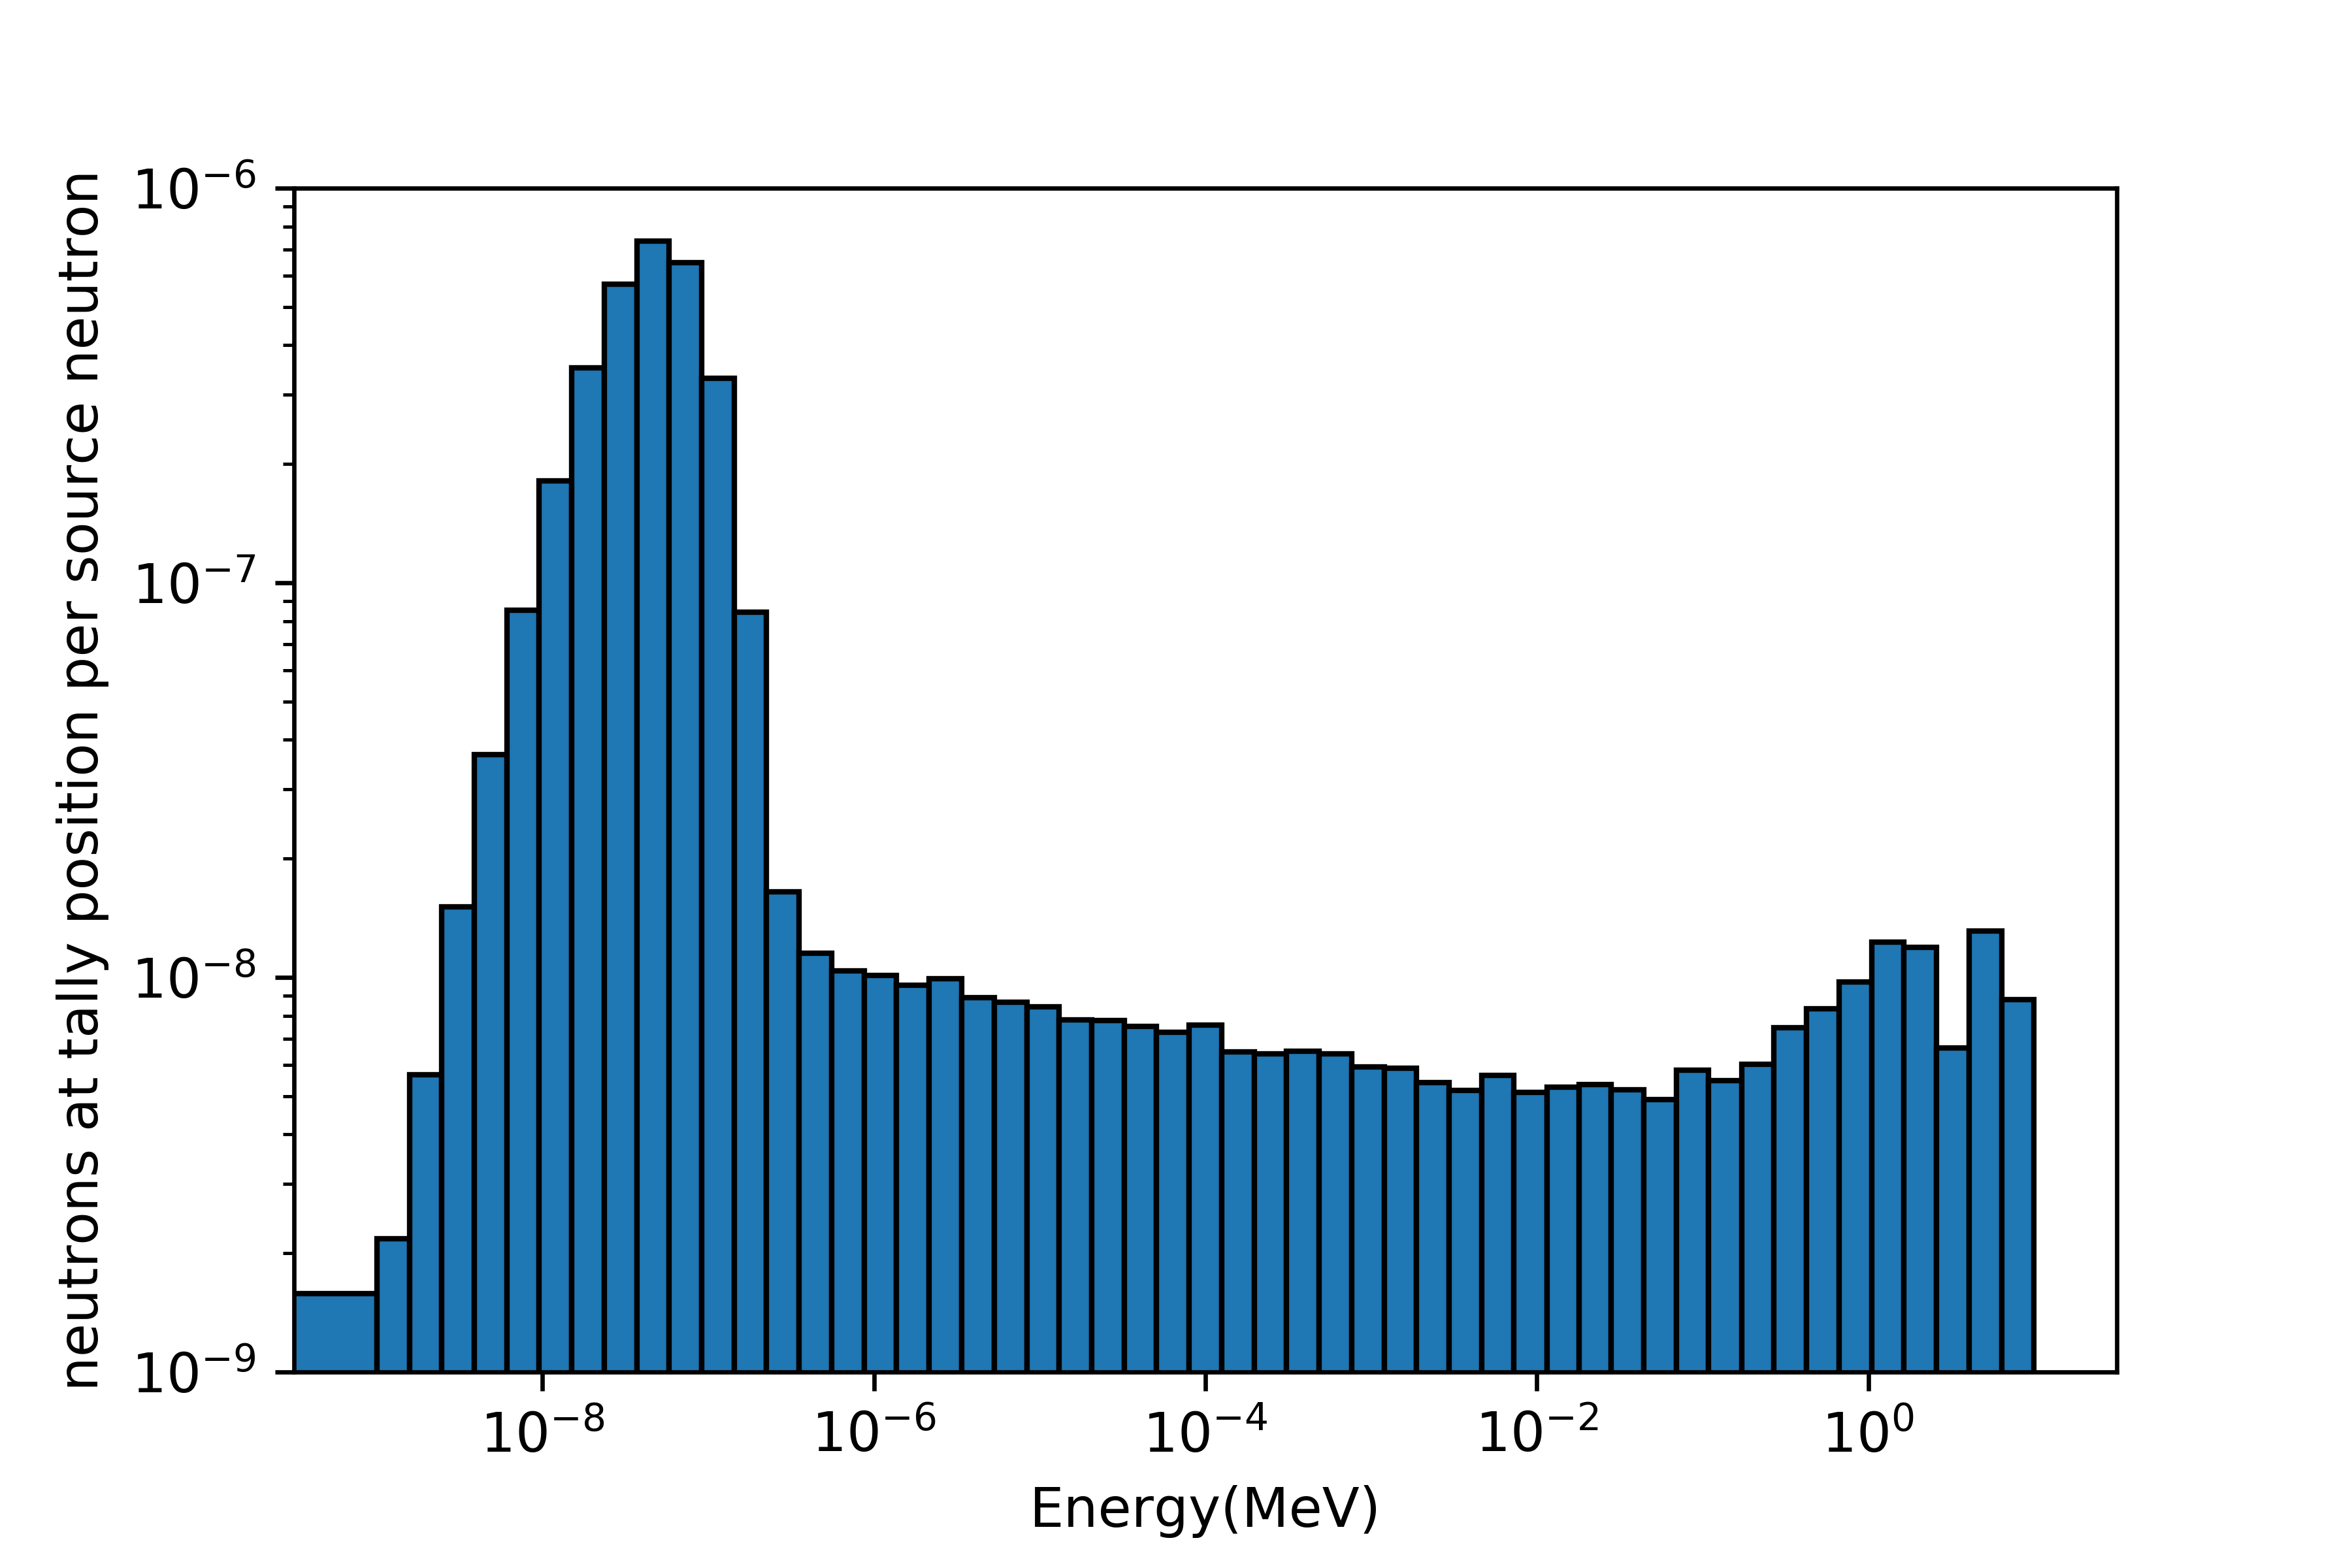
\includegraphics[height=5cm]{hist.png}
    \caption{Probability for the distribution of neutron energies reaching the detector from the middle of the stack \cite{Ben}}
    \label{fig:prob}
\end{figure}
\subsection{Results-1\,bar}
The run selected for 1\,bar was at 3800V which from the gain study would equate to a gain of around 11. The details of the experimental run can be found in Table \ref{tb:1bar}, with H1 being the voltage on the far channel and H2 the voltage on the near channel. This voltage difference is chosen due to the differing gains between the two channels caused by the manufacturing process allowing for the neutron peak to occur at or around the same amplitude on both channels. The trigger is selected to remove a portion of the low amplitude noise at the time of acquisition.
\begin{table}[H]
\centering
\caption{Experimental information for 1 bar run}
\begin{tabular}{|l|l|l|l|l|l|l|} 
\hline
\begin{tabular}[c]{@{}l@{}}Gas Pressure\\(Bar)\end{tabular} & \begin{tabular}[c]{@{}l@{}}H1\\(V)\end{tabular} & \begin{tabular}[c]{@{}l@{}}H2\\(V)\end{tabular} & Events & \begin{tabular}[c]{@{}l@{}}Time\\(s)\end{tabular} & \begin{tabular}[c]{@{}l@{}}Rate\\(Hz)\end{tabular} & \begin{tabular}[c]{@{}l@{}}Trigger\\(ADU)\end{tabular}  \\ 
\hline
1                                                          & 3800                                            & 3724                                            & 437310 & 20574                                             & 21.26                                              & 50                                                      \\
\hline
\end{tabular}
\label{tb:1bar}
\end{table}
\noindent The raw data produced from the run is shown in Figure \ref{fig:ampb}, with a total rate of $9.91\,Hz$ on the near and $11.34\,Hz$ on the far channel. To remove the low amplitude noise, cuts on the characteristics of the pulse are used with the cuts being independently chosen. The 2D histogram for the rise time is shown in Figure \ref{fig:1rise}, and multiple regions can be found. The rise time is affected by the incident particle and the length of the ionising track. The low amplitude peak has a high density region with rise time between 0.3-0.6\,ms, however the extremely dense region centered around 0.5ms is an overflow from the analysis software that is yet to be fixed. 
\newline Particularly observed in the far channel, is a region of around 250\,ADU that was believed to be the thermal neutron peak. To ensure that this region was produced by physical events or neutrons, multiple pulses were checked within and around the region. This was done by checking the proportionality between the height and the fall and comparing pulses within the region with pulses from outside the region.
\begin{figure}[H]-
    \centering
    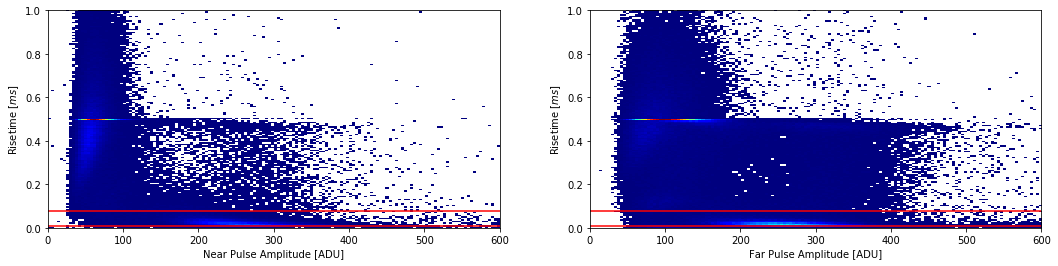
\includegraphics[height=3.7cm]{uk24n001_rise.png}
    \caption{2D histogram of amplitudes vs rise time at 3800V, 1\,bar}
    \label{fig:1rise}
\end{figure}
\noindent The rise time removes a large majority of the low amplitude peak but is not very precise as the neutron region is quite broad, which allows for low rise time noise to remain. Figure \ref{fig:1fall} shows the 2D histogram for the amplitude vs fall of the pulse and was a good remover of the low amplitude noise as well as events around the neutron amplitudes especially in the near channel with majority of the dense region falling outside the cut region.
\begin{figure}[H]-
    \centering
    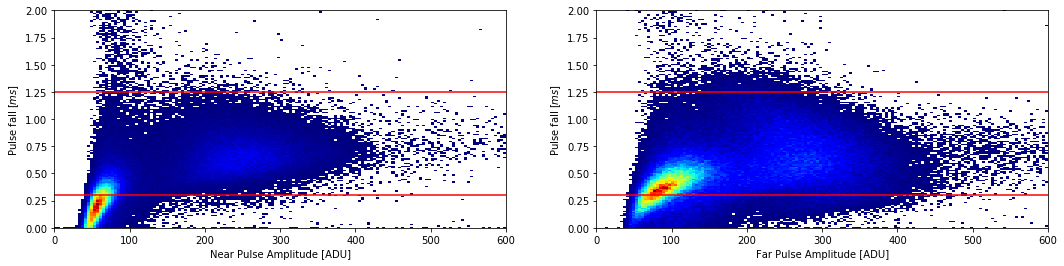
\includegraphics[height=3.7cm]{uk24n001_fall.png}
    \caption{2D histogram of amplitude vs fall at 3800V, 1\,bar}
    \label{fig:1fall}
\end{figure}
\noindent The cuts on both channels are the same on this run as both channels are very similar, but they are selected individually, shown later on at higher pressures. The regions in Figures \ref{fig:1fall}, \ref{fig:1dur} are very broad, suggesting that the fall and duration varies considerably more for the same pulse height which allows for the lower amplitude noise to remain.
\begin{figure}[H]- 
    \centering
    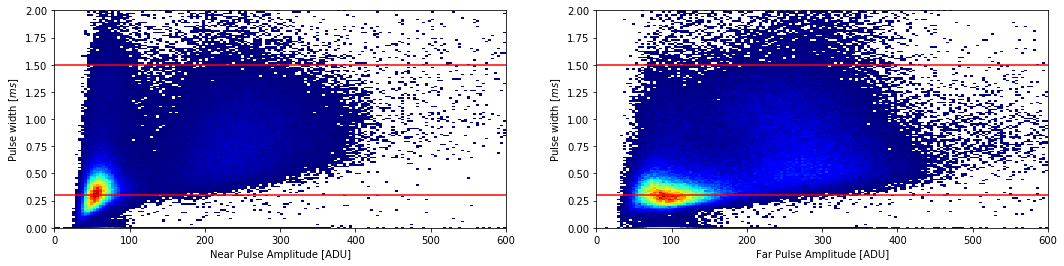
\includegraphics[height=3.7cm]{uk24n001_dur.png}
    \caption{2D histogram of amplitude vs duration at 3800V, 1\,bar}
    \label{fig:1dur}
\end{figure}
\begin{figure}[H]-
    \centering
    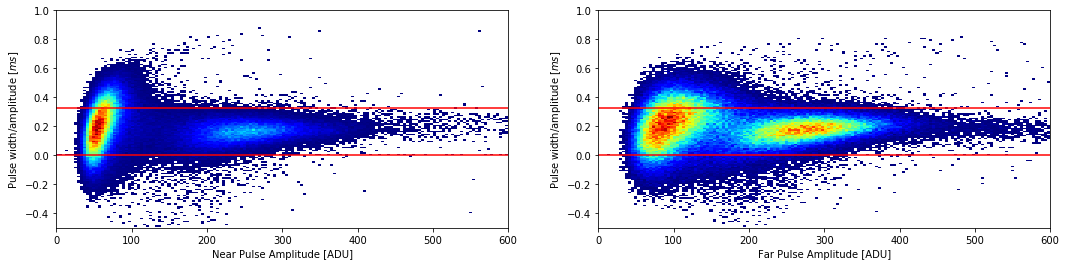
\includegraphics[height=3.7cm]{uk24n001_len.png}
    \caption{2D histogram of amplitude vs ratio at 3800V, 1\,bar}
    \label{fig:1len}
\end{figure}
\noindent Table \ref{tb:1cuts} contains the cuts applied on the characteristics of the pulse and can be compared to other measurements at different pressures and voltages.
\begin{table}[H]
\centering
\caption{Experimental information for 1 bar run}
\begin{tabular}{|l|l|l|l|l|l|l|l|} 
\hline
\multicolumn{2}{|l|}{Rise Time~~ } & \multicolumn{2}{l|}{Pulse Width~~ } & \multicolumn{2}{l|}{Pulse Fall~~ } & \multicolumn{2}{l|}{Pulse width/amplitude~~ }  \\ 
\hline
Min                         & Max  & Min                     & Max       & Min                     & Max      & Min                   & Max                    \\ 
\hline
\multicolumn{1}{|l}{0.0075} & 0.07 & \multicolumn{1}{l}{0.3} & 1.5       & \multicolumn{1}{l}{0.3} & 1.25     & \multicolumn{1}{l}{0} & 0.325                  \\
\hline
\end{tabular}
\label{tb:1cuts}
\end{table}
\noindent The combination of all the cuts produced the plot in Figure \ref{fig:1aft}, which removed most of the low amplitude peak and didn't impact the neutron peak. As previously stated the channels have multiple anodes connected with differing gains, which produces peaks at multiple amplitudes. A single Gaussian would not describe the peak accurately, and so multiple peaks describing each anode could be used. However this would over complicate the combination of the peaks, so a weighted double Gaussian was chosen. 
\begin{equation}
     f(x) = A_1\frac{exp(\frac{\frac{x-\mu_1}{\sigma_1}}{2})}{\sqrt{2\pi}} + A_2\frac{exp(\frac{\frac{x-\mu_2}{\sigma_2}}{2})}{\sqrt{2\pi}}
\end{equation}
The mean of the weighted Gaussian is calculated using 
\begin{equation}
    \mu_c = \frac{A_1}{A_1+A_2}\mu_1 + \frac{A_2}{A_1+A_2}\mu_2  
\end{equation}
and the standard deviation of the weighted Gaussian \cite{tzamarias}:
\begin{equation}
    \sigma_c^2 = \left(\frac{A_1}{A_1+A_2}\right)^2\sigma_1^2 + \left(\frac{A_2}{A_1+A_2}\right)^2\sigma_2^2 + \left(\frac{A_1}{A_1+A_2}\right)\left(\frac{A_2}{A_1+A_2}\right)(\sigma_1^2+\sigma_2^2+(\mu_1 - \mu_2)^2)
\end{equation}
\begin{figure}[H]- 
    \centering
    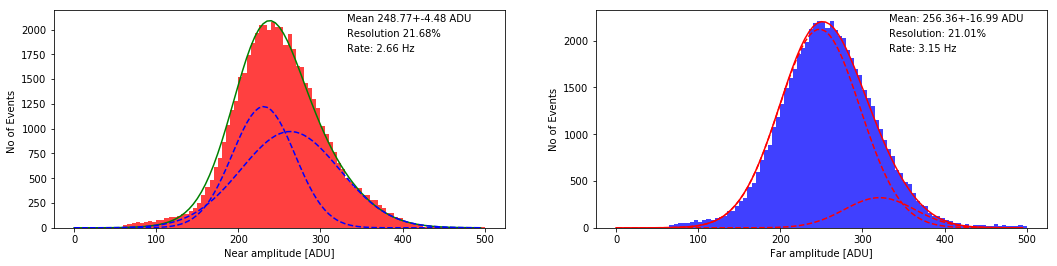
\includegraphics[height=3.7cm]{uk24n001_amp.png}
    \caption{Neutron peak for 3800V at 1\,bar after cuts on the characteristics of the pulse}
    \label{fig:1aft}
\end{figure}
\noindent The error was calculated using the same method and was taken from the error on the estimation on the constants of the Gaussian fit. The double Gaussian fit on the near channel describes the peak accurately with the two Gaussian's displaying similar scales and height. The accuracy of the fit can be quantified using the $chi^2$ method:
\begin{equation}
   \frac{\chi^2}{d_{of}} =  \frac{(y_c-y_o)^2}{y_od_{of}}
   \label{eq:chi}
\end{equation}
$d_{of}$ is the degrees of freedom or the number of points calculated, $y_c$ is the calculated y value of the Gaussian and $y_o$ is the observed y value.
\newline Using this, the accuracy can be quantified as $\frac{\chi^2}{d_{of}} = 4.28$. A perfect fit would have a value of 1 meaning that the fit is overestimating the peak slightly but does not deviate significantly. The neutron peak in the near channel had a mean of $248.77 \pm 4.48$\,ADU with a resolution of $21.68$\,\% and rate of $2.66$\,Hz. The cuts have removed $73$\,\% of the events on the near channel and have removed the large low amplitude peak. However the cuts are not guaranteed to remove 100\% of the unwanted events around the neutron peak.
\newline The double Gaussian fit on the far channel seems to be a good fit visually with the majority of events described with one Gaussian with a small contribution from a higher amplitude peak. This is quantified using Equation \ref{eq:chi}, $\frac{\chi^2}{d_{of}} = 4.53$, suggesting there is some deviation but is comparable to the result for the near channel.
The far channel had a mean of $256.36 \pm 16.99$\,ADU with a resolution of $21.61\%$ and rate of $3.15$\,Hz, with $71$\,\% of total events being removed during the cuts. Using Equation \ref{eq:gain} the gain is estimated to be $11.5$ which is quite low and will allow for much higher neutron energies to fit within the limits of the detector.
\newline When comparing the plots in Figure \ref{fig:1aft}, in the near channel the double Gaussian peaks are closer together, resulting in the error of the mean being lower than that of the far channel. The amplitudes are very similar and are within the error of each other suggesting that the voltage difference is compensating correctly.
\newline The total rate between the two channels contains simultaneous events. These are not shared events  between the channels, as that would produce events that were half the energy (or amplitude) of the neutron peak. The simultaneous events are shown in Figure \ref{fig:1sym}\,a) and are centered around the amplitude of the neutron peak.
\begin{figure}[H]- 
    \centering
    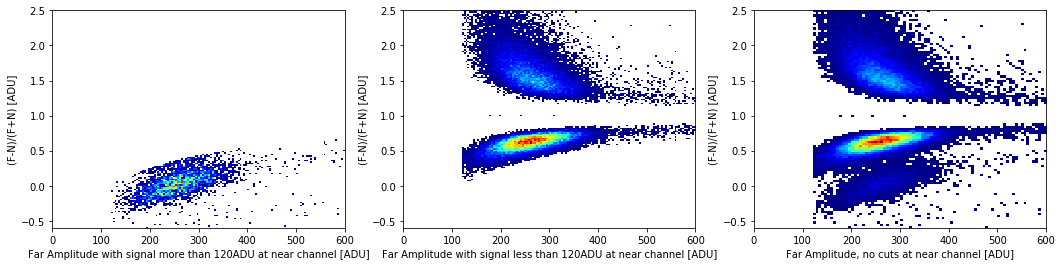
\includegraphics[height=3.7cm]{uk24n001_symgood.png}
    \caption{Symmetry plots vs far channel for 3800V at 1\,bar. a)Events that triggered on both channels, b) events that are only triggered on the far channel, c) total symmetry for the far channel}
    \label{fig:1sym}
\end{figure}
\noindent The calculated simultaneous events rate was $0.63$\,Hz and was removed from the rate calculated from Figure \ref{fig:1aft} to produce a total detection rate of $5.18$\,Hz. This resulted in an efficiency of $7.66\times10^{-04}$ which is an improvement from previous studies and allows in future to calculate the rate of an unknown source.
\newline For 1\,bar the detector has been calibrated, shown in Section \ref{calib} and i was possible to convert the amplitude to energy, shown in Figure \ref{fig:1ev}. The mean energy of the peak is $625.91 \pm 162.84$\,keV, which is close to the expected energy from Equation \ref{eq:neu}. The error is calculated using Equation \ref{eq:error} is considerable and could be improved by more energy points on the calibration plot. The histogram is again described with the double Gaussian, with the separate peaks being very similar to that of Figure \ref{fig:1aft}
\begin{figure}[H]- 
    \centering
    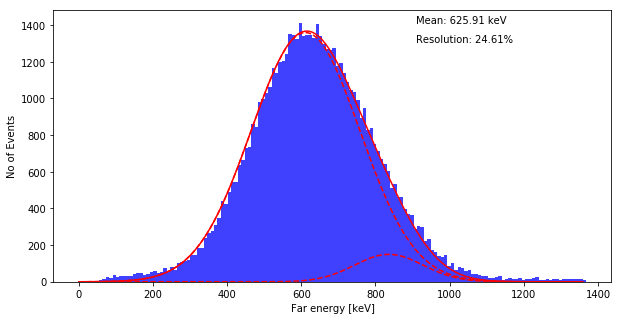
\includegraphics[height=3.7cm]{uk24n001_ev.png}
    \caption{Histogram for neutron energy on the far channel for 3800V at 1\,bar}
    \label{fig:1ev}
\end{figure}
\subsection{Results-1.5\,bar}
\begin{table}[H]
\centering
\caption{Experimental information for 1.5\,bar run}
\begin{tabular}{|l|l|l|l|l|l|l|} 
\hline
\begin{tabular}[c]{@{}l@{}}Gas Pressure\\(Bar)\end{tabular} & \begin{tabular}[c]{@{}l@{}}H1\\(V)\end{tabular} & \begin{tabular}[c]{@{}l@{}}H2\\(V)\end{tabular} & Events  & \begin{tabular}[c]{@{}l@{}}Time\\(s)\end{tabular} & \begin{tabular}[c]{@{}l@{}}Rate\\(Hz)\end{tabular} & \begin{tabular}[c]{@{}l@{}}Trigger\\(ADU)\end{tabular}  \\ 
\hline
1.5                                                         & 4500                                            & 4410                                            & 1080963 & 43239                                             & 35.8                                                 & 50                                                      \\ 
\hline
1.5                                                         & 4800                                            & 4704                                            & 1184166 & 18000                                             & 10.23                                              & 50                                                      \\
\hline
\end{tabular}
\end{table}
Two voltages were taken at 1.5\,bar, one at 4500\,V and one at 4800\,V. The 4800\,V run however failed to acquire past 4000 seconds resulting in minimal statistics so was discarded. The raw data shown in Figure \ref{fig:2bef} has a considerable low amplitude peak, with the neutron peak being around 900\,ADU. Compared to the raw data from the 1\,bar results in Figure \ref{fig:ampb} the neutron peak is about double the amplitude and much smaller in comparison to the noise peak. The rate on the near channel was $16.7$\,Hz and rate on the far channel was $19.1$\,Hz. 
\begin{figure}[H]- 
    \centering
    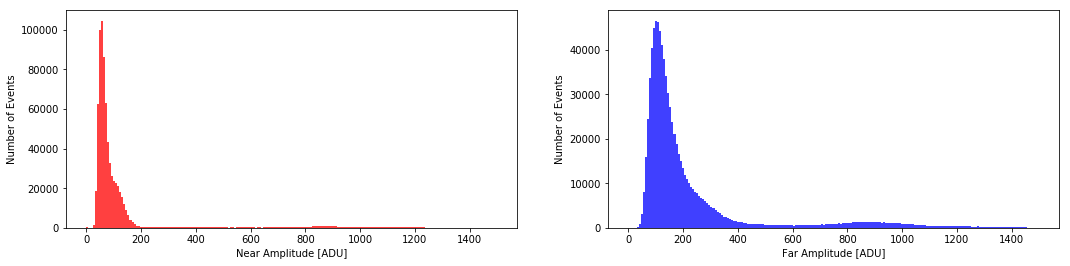
\includegraphics[height=3.7cm]{uk24n002_ampbefore.png}
    \caption{Raw data from 4500V at 1.5\,bar}
    \label{fig:2bef}
\end{figure}
\noindent The large low amplitude peak is slightly different to that of 1\,bar, with a small foot at the bottom. Analysing the amplitude vs time in Figure \ref{fig:2tim}, it shows electronic discharge at the start and end of the run. This could be removed with a time cut between 7000-21000 seconds, although this would result in lost neutron events, so normal cuts were used to try and remove this to isolate the neutron peak.
\begin{figure}[H]- 
    \centering
    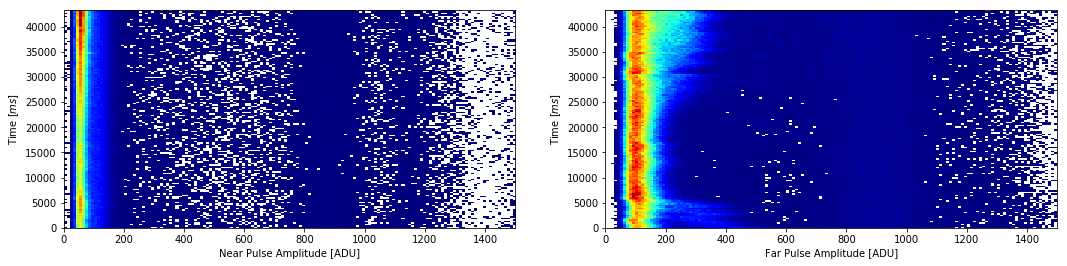
\includegraphics[height=3.7cm]{uk24n002_time.png}
    \caption{amplitude against time from 4500V at 1.5\,bar}
    \label{fig:2tim}
\end{figure}
\noindent The regions in the rise time plot in Figure \ref{fig:2rise} are more separated than those in Figure \ref{fig:1rise}, with more defined regions due to the higher pressure reducing the length of the ionising track. There are two regions that contribute to the low amplitude peak. One occurs at low rise time that is included in the cut which is most likely either produced by a neutron that has not fully dissipated it energy in the volume of the detector or the electrical discharge that is occurring in the detector and another large region between 0.4 and 0.8 milliseconds which is possibly electrical noise.
\begin{figure}[H]-
\centering
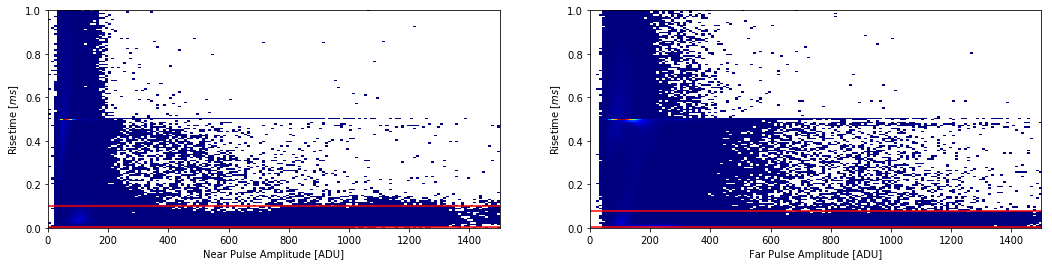
\includegraphics[height=3.7cm]{uk24n002_rise.png}
\caption{2D histogram of amplitudes vs rise time at 3500V, 1.5\,bar}
\label{fig:2rise}
\end{figure}
\noindent The 2D histogram in Figure \ref{fig:2fall} had to have more checks than other cuts due to the large region in the far channel under the lower red cut line which is not present in the near channel. Multiple pulses were checked below the cut line, which looked very different to that of the pulses in the cut region and so were removed using the cut. This cut was very efficient at cutting the low amplitude noise with the densest region falling outside of the cut area.
\begin{figure}[H]-
\centering
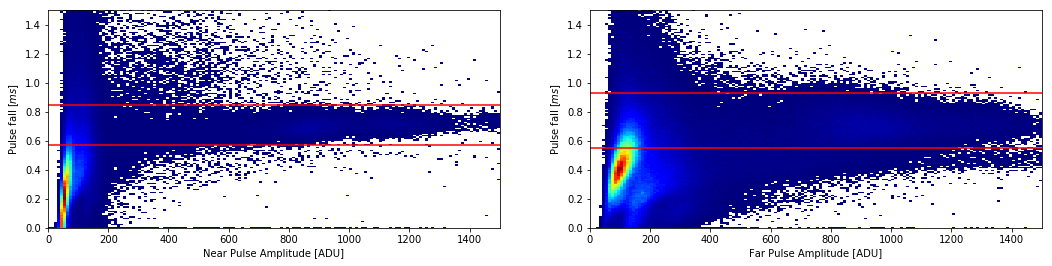
\includegraphics[height=3.7cm]{uk24n002_fall.png}
\caption{2D histogram of amplitudes vs fall at 3500V, 1.5\,bar}
\label{fig:2fall}
\end{figure}
\noindent The cut region on the far channel in Figure \ref{fig:2dur} is much larger than the cut region on the near which allows for more unwanted events to pass through the cut. However compared to Figure \ref{fig:2fall} there is no distinct separate regions in this area.
\begin{figure}[H]-
\centering
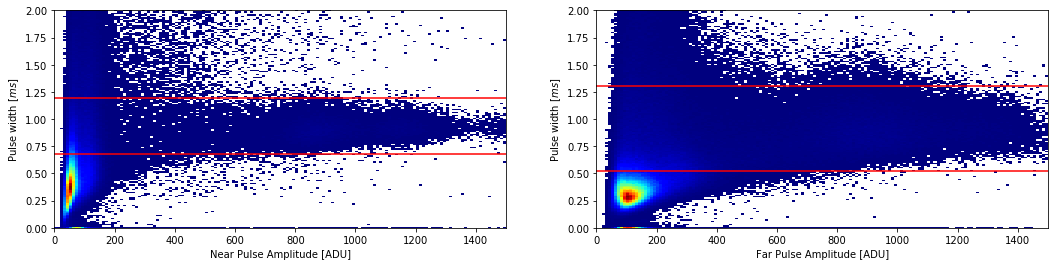
\includegraphics[height=3.7cm]{uk24n002_dur.png}
\caption{2D histogram of amplitudes vs duration at 3500V, 1.5\,bar}
\label{fig:2dur}
\end{figure}
\noindent The ratio cut in Figure \ref{fig:2len} was very efficient at removing the unwanted events because the long thin region allowed for a large portion of the dense region at low amplitude being removed.
\begin{figure}[H]-
    \centering
    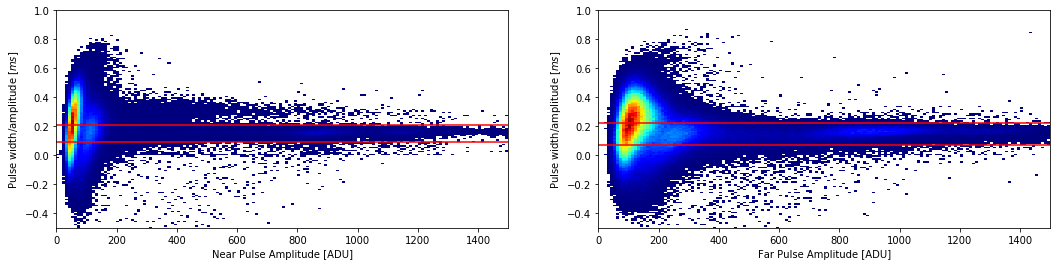
\includegraphics[height=3.7cm]{uk24n002_len.png}
    \caption{2D histogram of amplitudes vs ratio at 3500V, 1.5\,bar}
    \label{fig:2len}
\end{figure}
\begin{table}
\centering
\caption{Cuts on data for 1.5\,bar run}
\label{tb:15bar}
\begin{tabular}{|l|ll|ll|ll|ll|} 
\cline{2-9}
\multicolumn{1}{l|}{} & \multicolumn{2}{l|}{Rise Time}   & \multicolumn{2}{l|}{Pulse Width} & \multicolumn{2}{l|}{Pulse Fall} & \multicolumn{2}{l|}{Pulse Ratio}  \\ 
\cline{2-9}
\multicolumn{1}{l|}{} & \multicolumn{1}{l|}{Min} & Max   & \multicolumn{1}{l|}{Min} & Max   & \multicolumn{1}{l|}{Min} & Max  & \multicolumn{1}{l|}{Min} & Max    \\ 
\hline
Far                   & 0.0055                   & 0.075 & 0.52                     & 1.3   & 0.55                     & 0.93 & 0.07                     & 0.22   \\ 
\hline
Near                  & 0.0055                   & 0.1   & 0.68                     & 1.19  & 0.57                     & 0.85 & 0.09                     & 0.21   \\
\hline
\end{tabular}
\end{table}
\noindent Comparing the histogram produced after the cuts with the raw data in Figure \ref{fig:2com}, the low amplitude peak is still comparable to the size of the neutron peak but has been reduced compared to the low amplitude peak in the raw data. This is most likely due to sparking within the detector (Figure \ref{fig:2tim}) which produced pulses that passed all of the cuts. Around the neutron peak the cuts have been very efficient, not removing excessive amounts of the peaks.
\begin{figure}[H]-
    \centering
    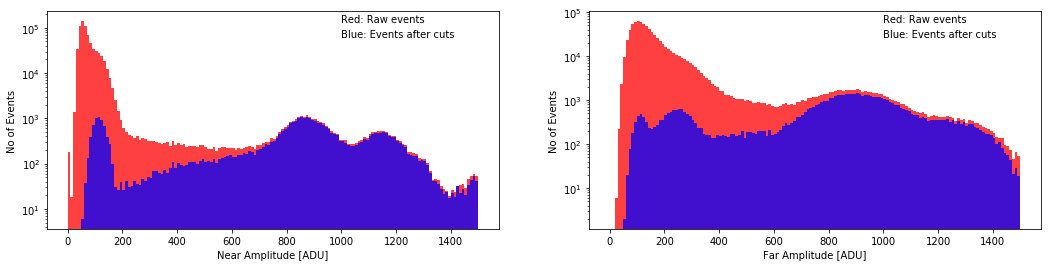
\includegraphics[height=3.7cm]{uk24n002_ampcomp.png}
    \caption{Histogram comparing cut data in blue with raw data in red at 3500V, 1.5\,bar}
    \label{fig:2com}
\end{figure}
\noindent The histogram in Figure \ref{fig:2amp} only displays the amplitude between 400-1500\,ADU to improve the accuracy of the Gaussian's plots. Due to the higher gain of around 39 compared to the 1\,bar result, the gains on the multiple anodes have separated enough to be separately visible in both the near channel and the far. From this, it is possible to deduce that the near channel has more variation between the anodes compared to the far channel, which can be mostly described by a single Gaussian with a small peak after that. In comparison, the near channel has two separated peaks in which the large peak is still described by a double Gaussian, suggesting there are still more peaks within this. The peak is quite sharp with a background of around 200 counts, resulting in a un-optimal fitting to the peak. However the far channel is much better and is the most likely one to be used for this run.
\newline The larger peak in the near channel had a mean of $876.15 \pm 11.33$\,ADU, with a resolution of $11.33$\,\% and a $\frac{\chi^2}{d_{of}} = 1.22$. The total rate of the neutron region was $0.95$\,Hz which was a reduction of 94.3\% which is much greater than the 1\,bar. 
\newline The double Gaussian in the far channel has a $\frac{\chi^2}{d_{of}} = 1.72$, however its mostly described by the first single Gaussian peak which has a amplitude of $893.67 \pm 1.43$\,ADU, with a resolution of $15.29$\,\%. The total rate of the neutron region was $1.6$\,Hz.
\begin{figure}[H]-
    \centering
    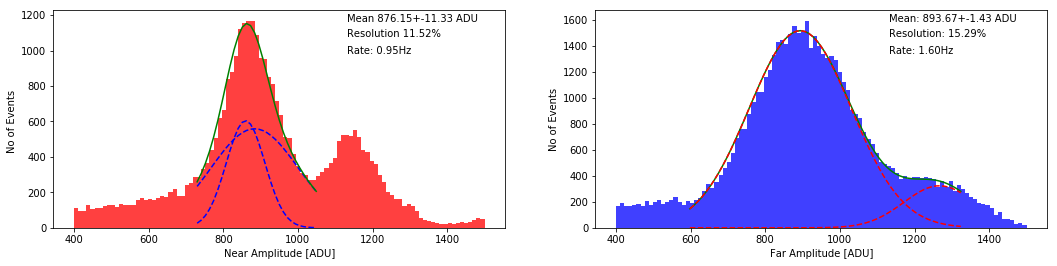
\includegraphics[height=3.7cm]{uk24n002_amp2.png}
    \caption{Amplitude histogram of cut data at 3500V, 1.5\,bar}
    \label{fig:2amp}
\end{figure}
\noindent The simultaneous event rate was calculated to be $0.16$\,Hz which is shown in Figure \ref{fig:2sym}, reducing the total detection rate to $1.92$\,Hz, which equated to an efficiency of $3.08\times 10^{-04}$ which has reduced slightly compared to 1\,bar .
\begin{figure}[H]-
    \centering
    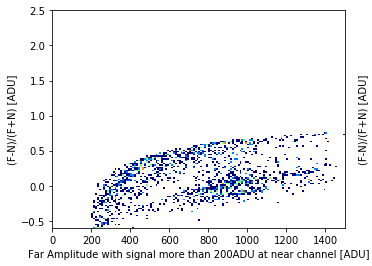
\includegraphics[height=3.7cm]{uk24n002_symcutgood1.png}
    \caption{2D histogram of amplitudes vs ratio at 3500V, 1.5\,bar}
    \label{fig:2sym}
\end{figure}
\subsection{Results-2\,bar}
\begin{table}[H]
\centering
\caption{Experimental information for 2\,bar run}
\label{tb:2bar}
\begin{tabular}{|l|l|l|l|l|l|l|} 
\hline
\begin{tabular}[c]{@{}l@{}}Gas Pressure\\(Bar)\end{tabular} & \begin{tabular}[c]{@{}l@{}}H1\\(V)\end{tabular} & \begin{tabular}[c]{@{}l@{}}H2\\(V)\end{tabular} & Events & \begin{tabular}[c]{@{}l@{}}Time\\(s)\end{tabular} & \begin{tabular}[c]{@{}l@{}}Rate\\(Hz)\end{tabular} & \begin{tabular}[c]{@{}l@{}}Trigger\\(ADU)\end{tabular}  \\ 
\hline
1.96                                                        & 4950                                            & 4851                                            & 187022 & 17165                                             & 10.9                                             & 50                                                      \\
\hline
\end{tabular}
\end{table}
\noindent The voltage selected for the run is at the limit of the electronics, which resulted in the neutron peak appearing closer to the large low amplitude noise peak shown in Figure \ref{fig:3bef} compared to the 1.5\,bar and is more comparable to the 1\,bar run. The rate in the near channel was $5.4$\,Hz and $5.5$\,Hz in the far channel.
\begin{figure}[H]-
    \centering
    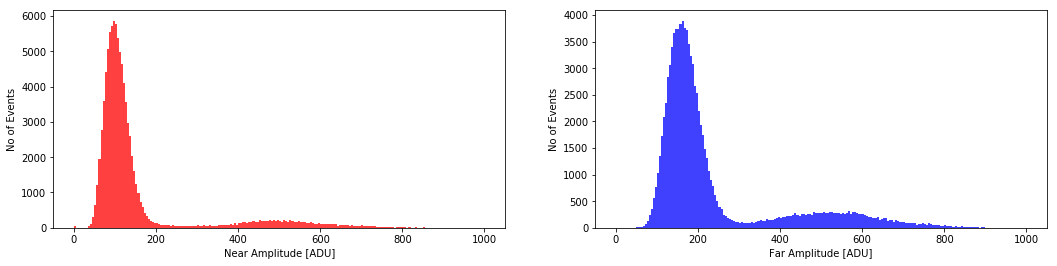
\includegraphics[height=3.7cm]{uk26n000_ampbefore.png}
    \caption{Raw data for 4950V, 2\,bar}
    \label{fig:3bef}
\end{figure}
\noindent Due to the higher pressure, the regions in Figure \ref{fig:3rise} are more separated with less events between the regions. Compared to the rise times for 1\,bar and 1.5\,bar in Figures \ref{fig:1rise} and \ref{fig:2rise}, the low amplitude low rise time region has greatly reduced. This is believed to be where interactions effected by the wall effect would be found, with comparable rise times to the neutrons but at a lower energy. This suggests that the higher pressure has reduced the length of the ionisation tract to a point where the probability of it hitting the wall before dissipating all of its energy is very low.
\begin{figure}[H]-
    \centering
    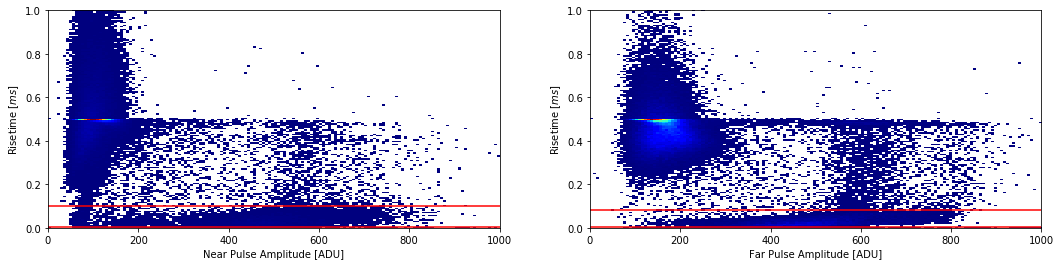
\includegraphics[height=3.7cm]{uk26n000_rise.png}
    \caption{2D histogram of amplitudes vs rise time for 4950V, 2\,bar}   
    \label{fig:3rise}
\end{figure}
\noindent However this has had negative effects in the fall plots shown in Figure \ref{fig:3fall}, with the region being more spread out and resulting in a cut that only removed minimal noise events. This suggests that as the pressure increases, the size of the exponential fall becomes more erratic and unpredictable. However, the fall is dependent on the electronics, which were being used at the voltage limit which possibly could be the reason for this and could be negated with higher voltage rated electronics.
\begin{figure}[H]-
    \centering
    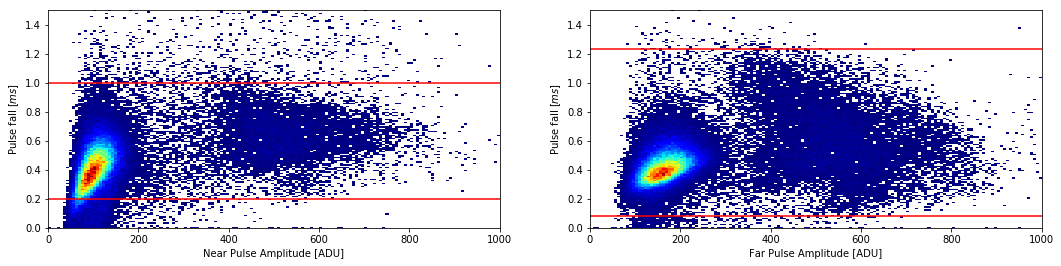
\includegraphics[height=3.7cm]{uk26n000_fall.png}
    \caption{2D histogram of amplitudes vs fall for 4950V, 2\,bar}
    \label{fig:3fall}
\end{figure}
\begin{figure}[H]-
    \centering
    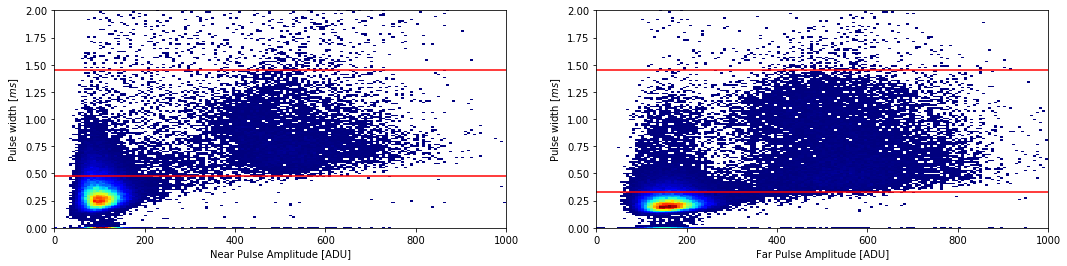
\includegraphics[height=3.7cm]{uk26n000_dur.png}
    \caption{2D histogram of amplitudes vs width  for 4950V, 2\,bar}
    \label{fig:3dur}
\end{figure}
\noindent The width around the neutron region is greater than that of the majority of the low amplitude noise peak resulting in the dense region falling outside of the cut, removing a large portion of the unwanted peak.
\newline The ratio plot also allows for a good cut to remove a portion of the low amplitude region, with a clear distinct region spread across the area of interest for the neutron peak. In future a diagonal amplitude cut could completely isolate then neutron region.
\begin{figure}[H]-
    \centering
    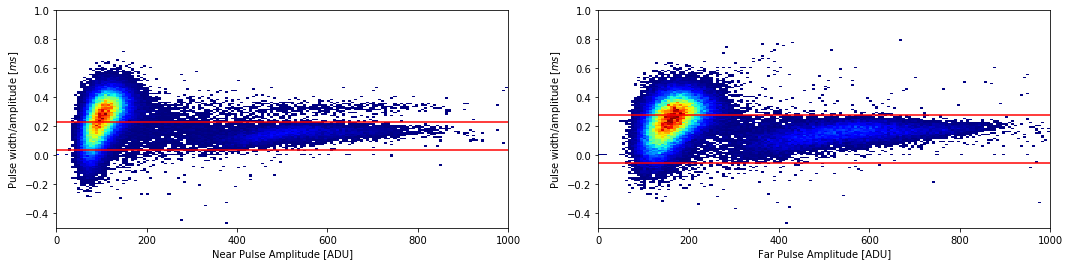
\includegraphics[height=3.7cm]{uk26n000_len.png}
    \caption{2D histogram of amplitudes vs ratio  for 4950V, 2\,bar}
    \label{fig:3len}
\end{figure}
\noindent Looking at Table \ref{tb:2bar}, other than the rise time, the cut regions on the other characteristics are much wider than on the near channel. This seems to be consistent with values from Table \ref{tb:15bar}, suggesting that the difference between the regions on each channel could be a result of the manufacturing process of the sensors. However these cuts are selected by eye and do come with an expected error which could account for this difference.
\begin{table}[H]
\centering
\caption{Experimental information for 2 bar run}
\label{tb:2bar}
\begin{tabular}{|l|ll|ll|ll|ll|} 
\cline{2-9}
\multicolumn{1}{l|}{} & \multicolumn{2}{l|}{Rise Time} & \multicolumn{2}{l|}{Pulse Width} & \multicolumn{2}{l|}{Pulse Fall} & \multicolumn{2}{l|}{Pulse Ratio}  \\ 
\cline{2-9}
\multicolumn{1}{l|}{} & \multicolumn{1}{l|}{Min} & Max                                   & \multicolumn{1}{l|}{Min} & Max                                     & \multicolumn{1}{l|}{Min} & Max                                    & \multicolumn{1}{l|}{Min} & Max                                                \\ 
\hline
Far                   & 0.004                    & 0.08                                  & 0.33                     & 1.45                                    & 0.31                     & 1.23                                   & 0.04                     & 0.26                                               \\ 
\hline
Near                  & 0.004                    & 0.1                                   & 0.48                     & 1.45                                    & 0.4                      & 1                                      & 0.04                     & 0.3                                                \\
\hline
\end{tabular}
\end{table}
\noindent The cuts produced the amplitude histogram are shown in Figure \ref{fig:3amp}, with the low amplitude peak completely removed, and just the neutron peak remaining. 
\newline The near channel was described with the double Gaussian, describing the peak well with similar Gaussian components as Figure \ref{fig:1aft} and has a chi squared of $1.41$ meaning that this is a good fit with a small overestimation. The weighted double Gaussian produced a mean of $500.11 \pm 4.39$\,ADU, a resolution of $22.34$\,\% and a rate of $0.44$\,Hz.
\newline In the far channel the double Gaussian fits the histogram well with a chi squared of $1.11$. However the data can be described by a single Gaussian for the most of the events, with a small second peak after that. The single Gaussian had a mean of $481.88 \pm 1.11$\,ADU, a resolution of $21.91$\,\% and a rate of $0.70$\,Hz. The resolution on both channels is comparable to the resolution of 1\,bar, suggesting that the 1.5\,bar results were affected by the electrical discharges.
\begin{figure}[H]-
    \centering
    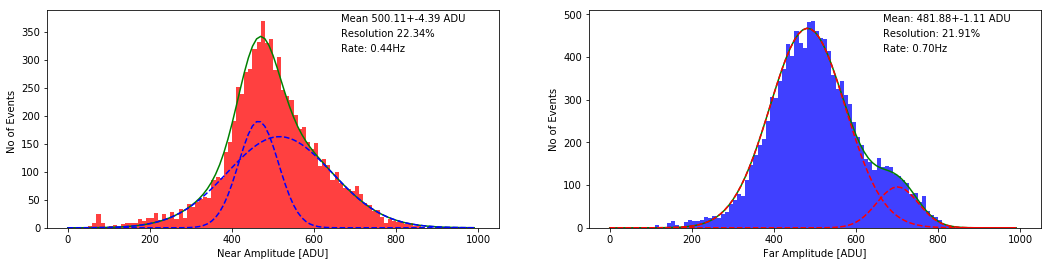
\includegraphics[height=3.7cm]{uk26n000_amp.png}
    \caption{Amplitude histogram of cut data for 4950V, 2\,bar}
    \label{fig:3amp}
\end{figure}
\noindent The simultaneous event rate was calculated to be $0.02$\,Hz, with these events shown in Figure \ref{fig:3sym} and was removed producing the total rate of $1.12$\,Hz, resulting in an efficiency of $1.65\times 10^{-04}$. This is smaller but comparable to 1\,bar even with a much lower count rate.
\begin{figure}[H]-
    \centering
    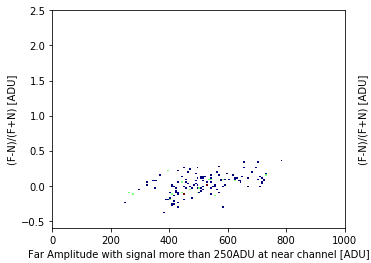
\includegraphics[height=3.7cm]{uk26n000_symcheck2.png}
    \caption{2D histogram of amplitudes vs ratio at 4950V, 2\,bar}
    \label{fig:3sym}
\end{figure}
\section{Conclusions}
\begin{table}[H]
\centering
\caption{Results from all three pressures on the far channel.}
\begin{tabular}{|l|l|l|l|l|} 
\hline
Pressure & Voltage & Estimated Gain & Detection Rate & Efficiency  \\ 
\hline
1       & 3800    & 11.5              & 5.18           & $7.66 \times 10^{-4}$      \\
1.5     & 4500    & 39              & 1.92           & $3.08 \times 10^{-4}$          \\
1.98    & 4950    & 21.6              & 1.12           & $1.65 \times 10^{-4}$          \\
\hline
\end{tabular}
\label{tb:fin}
\end{table}
During the project, the detector has been characterised by calculating the gain at multiple voltages, producing a plot showing the three regions the detector can be operated in, at a pressure of 1\,bar. When selecting the ionisation region the w value was calculated for nitrogen as $36.84 \pm 0.04$, a deviation of 0.45 from the known value. The detector was calibrated at 1\,bar to allow for energy conversion, shown in Figure \ref{fig:1ev}. Unfortunately these preliminary experiments were only done at 1\,bar which in future will have to be carried out a 1.5 and 2\,bar to understand how the detector is effected by the higher pressures, however it was possible to calculate the individual gains for each run.
\newline The neutron measurements at 1 and 2\,bar, successfully removed the majority of the noise using the multiple cuts. The 2\,bar experiment has shown that the wall effect could be negated by increasing the pressure, which in turn reduces the size of the ionisation track. This can been seen when comparing the two rise time 2D histograms in Figures \ref{fig:1rise} and \ref{fig:3rise}, with the low amplitude, low rise time region disappearing as the pressure increased. The 2\,bar result was a break though with no other experiments showing the feasibility of neutron measurements using a SPC filled with nitrogen at high pressures. Due to the maximum voltage rating for the electronics, the possibility of doing multiple runs to compare was not possible due to the already low gain at around 5\,kV. This maximum voltage has also limited the pressure to 2\,bar and higher pressures would require an upgrade to the electronics. The 1.5\,bar results were disappointing with large electronic discharges during the runs, producing a much greater amount of noise that could not be removed using the cuts. This did however show the presence of multiple peaks produced from the multiple anodes connected to the channels.
\newline The efficiencies between the pressures in Table \ref{tb:fin} show that as the pressure increases the efficiency has decreased slightly. However the voltage for 2\,bar is low and increasing this could increase the efficiency. To be sure multiple pressures at similar gains would have to be produced but this is still an improvement upon previous studies.
\newline The results have shown the feasibility of thermal neutron spectroscopy at reasonably low amplitudes, suggesting the possibility of fast neutron spectroscopy needed to encapsulate the entire background neutrons produced from the environment. A fast neutron study would have to be carried out in underground laboratory such as Boulby, due to the higher energy neutrons.
\newline The process of selecting cuts was very time consuming for each run. For experiments with large amount of runs this would take an unreasonable amount of time, so in future an algorithm could be produced to allow the decisions on the cuts to be automated and allow for a greater amounts of runs to be analysed at a time.
\section{Acknowledgements}
Many thanks to the NEWS-G group located in Birmingham, especially to my supervisors Kostas Nikolopoulos and Ioannis Katsioulas and especially Ioannis Manthos, for providing guidance and help through the course of the project. Also many thanks to my project partner Sam Green for helping with the workload and for giving me guidance.
\newpage

\bibliographystyle{IEEEtran}
\bibliography{ref} 

\newpage
%TC:ignore
\begin{appendix}
  \listoffigures
  \listoftables
  \section{Nuclei Decays}
    \subsection{Americium 241 Alpha Decay} \label{ap:a1}
        \begin{figure}[H]-
        \centering
        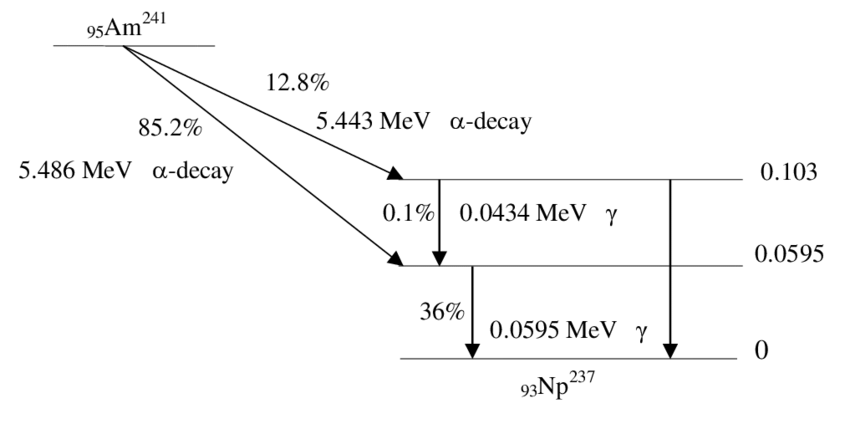
\includegraphics[height=5cm]{Am241.png}
        \caption{Alpha decay of Americium-241 \cite{Malain_2019}}
        \end{figure}
    \subsection{Polonium 210 Alpha Decay} \label{ap:a1}
        \begin{figure}[H]-
        \centering
        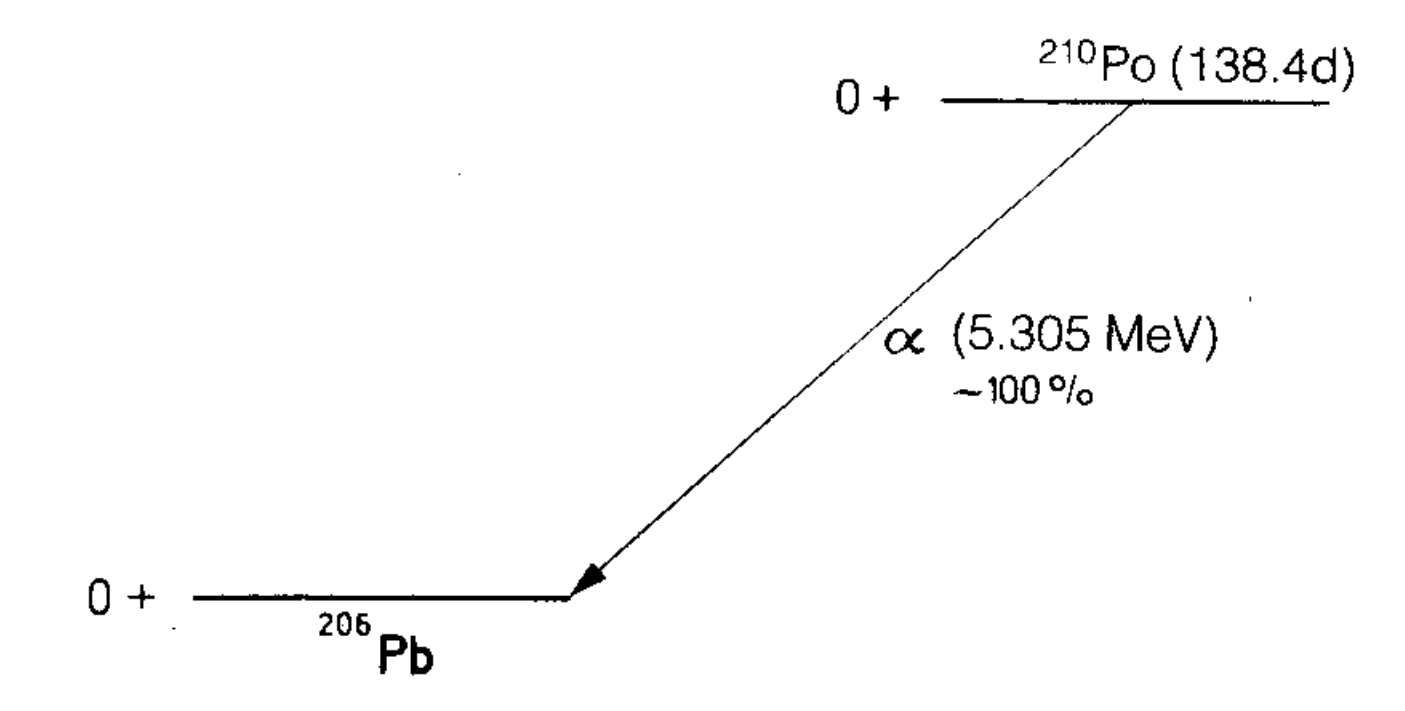
\includegraphics[height=5cm]{po210.png}
        \caption{Alpha decay of Polonium-241 \cite{lieser_2001}}
        \end{figure}
    \subsection{Decay chain of radon 222} \label{ap:a2}
        \begin{figure}[H]-
        \centering
        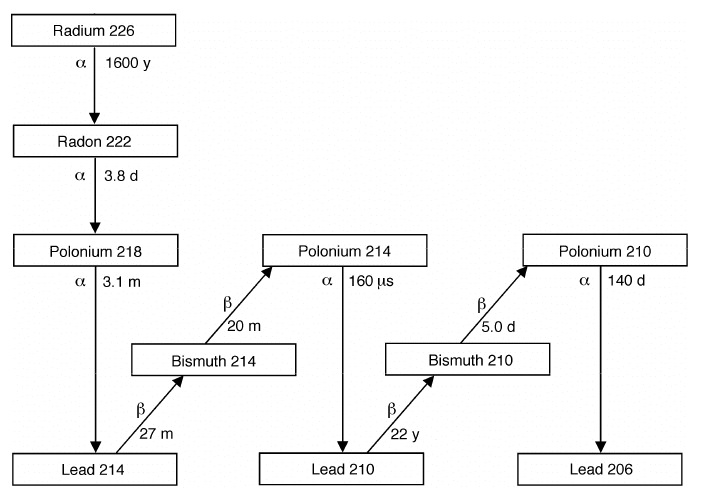
\includegraphics[height=5cm]{radon222.png}
        \caption{Decay chain of radon 222 \cite{nhess-10-2051-2010}}
        \end{figure}
    \section{Repository}
    All work including presentations, python code, ntuple files and excel data sheets can be found in the repository: \url{https://drive.google.com/drive/folders/1wTu-hEFVb-BicJJruVL6OvGmrak4dCtB?usp=sharing}
\end{appendix}
%TC:endignore
\newpage
%TC:ignore
%\quickwordcount{main}
%\quickcharcount{main}
%\detailtexcount{main}
%TC:endignore
\end{document}
